\documentclass[10pt]{jsreport}
\usepackage{graphicx}
\usepackage{braket}
\usepackage{bm,latexsym,amsmath,amssymb,amsfonts,mathrsfs}
\usepackage{amsthm}
\usepackage{bm}
\usepackage{tensor}
\usepackage{comment}
%\usepackage{physics}
\usepackage[dvipdfmx,linktocpage=true]{hyperref}
\usepackage{pxjahyper}
\usepackage[dvipdfmx]{color}
\usepackage{here}
\usepackage{tikz}
\usetikzlibrary {arrows.meta}
\usetikzlibrary {bending}
\input{colordvi.tex}
\usepackage{xcolor}%色
\usepackage{ulem}

\usepackage{ascmac}
\usepackage{framed}
\usepackage{tcolorbox}%式に色
\tcbuselibrary{theorems}
\tcbuselibrary{theorems,skins}

\setcounter{tocdepth}{3}%目次にsubsubsectionまで入れる
\setcounter{secnumdepth}{3}%1.a.b.cのように見出し番号をつける

\theoremstyle{definition}%定理環境の定義
\newtheorem{thm}{定理}[section]%これで(セクション番号.定理番号)という感じになる。

\newcommand{\kakko}[1]{\left(#1 \right)} %丸括弧()
\newcommand{\kkakko}[1]{\left[ #1 \right]} %角括弧[]
\newcommand{\nkakko}[1]{\left\{ #1 \right\}} %波括弧{}
\newcommand{\p}[1]{\left| #1 \right|} %縦棒||
\newcommand{\henbi}[2]{{\frac{\partial#1}{\partial#2}}} %偏微分
\newcommand{\bi}[2]{{\frac{d #1}{d #2}}} %微分

\newcommand{\del}{{\partial}} %偏微分の∂
\newcommand{\skakko}[1]{$\ll$#1$\gg$}
\newcommand{\vc}[1]{\overrightarrow{#1}}% 矢印ベクトル
\newcommand{\vct}[1]{\bm{#1}}%太字ベクトル
\newcommand{\sint}[1]{\int\mathcal{D}#1\,}%経路積分
\newcommand{\pms}[1]{\mathcal{D}#1\,}%経路積分の測度

%\newcommand{\Res}{\mathrm{Res}}
\renewcommand{\Im}{\mathrm{Im\,}}
\renewcommand{\Re}{\mathrm{Re\,}}
\DeclareMathOperator*{\Res}{Res}
\newcommand{\Tr}{\mathrm{Tr\,}}
\newcommand{\tr}{\mathrm{tr\,}}
\newcommand{\rank}{\mathrm{rank\,}}


\renewcommand{\prechaptername}{第}
\renewcommand{\postchaptername}{部}
%\renewcommand{\thechapter}{\roman{chapter}}

\renewcommand{\theenumi}{\Alph{enumi}}%アルファベットにする
\renewcommand{\labelenumi}{(\theenumi)}

\numberwithin{equation}{section}%数式番号を(n.m)の形で書く。

\topmargin=0.0in
\headsep=0.0in
\headheight=0.0in
\oddsidemargin=-0.22in
\evensidemargin=-0.22in
\textwidth=6.5in
\textheight=9.0in
\title{AI入門としての線形代数}
\author{TiroDuetto}
\date{\today}
\pagestyle{plain}

\begin{document}
\maketitle

\begin{abstract}
表題にはAI入門と銘打ってあるが私がAIについて詳しくないので、ほとんど線形代数の基本的な部分を記す。
一応計算機による解析も勉強していくつもりであり、このノート内でもできる限り具体例を提示していきたい。
内容はまだ書きかけなので随時更新していく。
もし重大な誤植や論理の間違いがあれば指摘してほしい。
なお、コンピュータとを計算機と呼んでいるのはそういう文化の人間が作った資料であるためであって深い意味はない。ゆえに表現が統一されていないところもあると思う。
このノートでは「我々が扱う空間は3次元Euclid空間であり、これは内積の定義された計量ベクトル空間である」という文章が理解できるところまで進めたら幸いと思う。
また、目次の5章と6章あたりの内容まで理解できれば計算機を用いた機械学習などにも応用できるだろうと期待している。
なお、このレジュメでは章立て\sout{がa.b.cのようになっているが、}\textcolor{red}{を1.a.b.cのようにした。}\footnote{documentclassをjsarticleからjsreportに変えたため。5/15変更。}aを章、bを節、cを項と呼んでいる。
\end{abstract}
\tableofcontents
\chapter{\underline{線形代数}}
\setcounter{section}{-1}
\section{数学的記法における注意}
\subsection{集合}
対象物の集まりを{\bf 集合}という。その集合を構成する対象物のことを{\bf 元}や{\bf 要素}という。集合$A$に元$a$が属することを
\begin{equation}
  a \in A 
\end{equation}
と書く。またすべてが$A$の元からなる集合$B$のことを、$A$の部分集合といい、
\begin{equation}
  B \subset A
\end{equation}
と書く。
\subsubsection{数の集合}
ある数全体の集合には特別な記号が用意されている。複素数$\mathbb{C}$, 実数$\mathbb{R}$, 有理数$\mathbb{Q}$, 整数$\mathbb{Z}$, 自然数$\mathbb{N}$など。
なお、この書体は黒板太字と呼ばれ、通常出版物において単なる太字である字を黒板で書くときに使われるが、以上の例のように特別な意味を持たせることもある。
もちろん出版物においては通常の太字で書いても問題はない。
例えば実数全体の集合を{\bf R}のように表している書籍もある。
\subsubsection{直積}
$c \in C, \, d\in D$を用いた$(c,d)$全体の集合のことを$C$と$D$の{\bf 直積}といい、$C\times D$と表す。例えば、座標平面上の点$(x,y)$は$\mathbb{R}\times \mathbb{R}$の元であると言える。なお、$\mathbb{R}\times \mathbb{R}=\mathbb{R}^{2}$とも書く。
\subsection{写像}
2つの集合があるとき、一方の集合の元に対して、もう一方の集合の元がただひとつに定まるような関係付けの規則を{\bf 写像}という。 
集合$V$から集合$W$への写像$f$を
\begin{equation}
  f:V \to W
\end{equation}
のように書く。あるいは元どうしの関係で$v\in V, \, w\in W$として
\begin{equation}
  v \mapsto w= f(v)
\end{equation}
と書く。$v \mapsto f(v)$と書いてもよい。大雑把に言えば$v$を入力したら$f$という規則によって$w$が出力されるということである。特に$V$や$W$が数の集合であれば、{\bf 関数}と呼ばれる。
\paragraph{例}
\begin{description}
  \item[実数から実数] 関数$y=f(x)$を以上の記法で表すと
  \begin{equation}
   f:\mathbb{R}\to\mathbb{R}, \quad x\mapsto y=f(x)
  \end{equation}
 \item[実数から複素数] 虚数単位$i=\sqrt{-1}$を用いて、$(x,y)\in \mathrm{R}^{2}$から複素数$z\in \mathbb{C}$を$z=g(x,y)=x+iy$のように定める。
 \begin{equation}
  g:\mathbb{R}^{2}\to \mathbb{C},\quad (x,y)\mapsto z=x+iy
 \end{equation}
 
\end{description}
\section{線形代数とは何か?}
世の中を大まかに把握したいとき、その現象を''真っ直ぐなもの''や''平らなもの''とみなしたり、単なる比例関係として扱うと便利だ。
例えば球体である地上に暮らしていても自分の近傍を平面とみなしたり、アルバイトによる収入も「毎月この程度」と簡単に近似して計算するだろう。
こういった考え方を「線形的に近似する」などと表現する。記憶にありそうな例で言えば、比例やその発展である1次関数である。
つまり、名前の通り「線形的な」対称を研究するのが線形代数というわけである。
また、代数という言葉は、簡単に言えば文字式による計算や方程式の研究する分野に用いられる。
合わせて「1次関数を研究する」学問と思っていて貰えばよい。
物理学においては本質的に非線形な現象であったとしても、そのうちの線形な部分を切り出して現象を理解したり、あるいは理論を構築していく。
\subsection{計算機において}
もともとはそういった動機から活かされていたのであるが、線形代数は奥が深く、応用範囲の広い分野である。
その重要な対称が{\bf ベクトル}や{\bf 行列}である。
今回の本題である計算機による解析では、いくつものデータをベクトルとして扱い、また新たなデータへの変換やその関係を行列で表す。$n$個のデータを$n$成分ベクトルで次のように表すとしよう
。\footnote{わかりやすさのために矢印でベクトルを表しているが、$\vc{v}$以外にも太字の$\vct{v}$やあるいは先にベクトルであると宣言した上で通常の$v$のまま表すこともある。物理をやっている人はこのあたりにこだわりがあるらしく、3次元は太字や矢印、4次元以上は特に明示せず、量子力学の文脈では$\ket{v}$などと書く。}
\begin{equation}
  \vc{v}=\left( \begin{matrix}
    v_{1}\\
    \vdots \\
    v_{n}
  \end{matrix} \right)
\end{equation}
このベクトルを$m$個のデータを表すベクトル$\vc{u}$に変換すると考える。
\begin{equation}
  \vc{v}=\left( \begin{matrix}
    u_{1}\\
    \vdots \\
    u_{m}
  \end{matrix} \right)
\end{equation}
単純計算でこの2つをつなげるためには$nm$個の成分を持つ変換が必要であるとわかるだろう。この変換を$A$と書けば
\begin{equation}
  A=\left( \begin{matrix}
    a_{11} & \cdots & a_{1n} \\
    \vdots & \ddots & \vdots \\
    a_{m1} & \cdots & a_{mn}
  \end{matrix} \right)
\end{equation}
これを用いて
\begin{align}
  \vc{u} &= A \vc{v}\\
 \Leftrightarrow  \left( \begin{matrix}
    u_{1}\\
    \vdots \\
    u_{m}
  \end{matrix} \right)&=\left( \begin{matrix}
    a_{11} & \cdots & a_{1n} \\
    \vdots & \ddots & \vdots \\
    a_{m1} & \cdots & a_{mn}
  \end{matrix} \right)\left( \begin{matrix}
    v_{1}\\
    \vdots \\
    v_{n}
  \end{matrix} \right)
\end{align}
このようにベクトル同士規則の変換を表すのが行列である。
そのまま$m\times n$行列と呼ばれる。この$m$や$n$の順序については後ほど説明する。
多数のデータを一度に扱いたい……それをきちんと定式化できたら……という願望を叶えてくれるのがこの計算である。
すでに線形代数で研究されつくされているのだ。
\subsubsection{例}
さて、以上の話は一般論に寄りすぎているし、まだベクトルも行列の話もしていない中では何をしているのか?という疑問のほうが大きいと思われるので簡単な例示をしていく。なお\cite{L-nakanishi}の例を少し改造しただけのものである。
いま、スーパーマーケットにいる。
桃、みかん、りんごの1個あたりの値段・重さの表\ref{momomikan}を知ったとき、果物を買った個数と合計の値段・重さの関係はどのように計算するのだろうか。
\begin{table}[H]
  \centering
  \caption{重さについては平均的な重さと思っておく。(例なのでそこまで重要でもないが)}
  \label{momomikan}
  \begin{tabular}{|c|c|c|c|} \hline
         & 桃 & みかん & りんご  \\ \hline
    値段(円)  & 300 & 100 & 200   \\ \hline
    重さ(g)  & 200 & 30 & 300  \\ \hline
  \end{tabular}
\end{table}


それぞれの果物を1個、2個、5個買ったとする。
もちろんこのときの計算は簡単で
\begin{align}
  (\text{値段})&=300\times 1 + 100\times 2+200\times 5 = 1500\\
  (\text{重さ})&= 200\times 1 + 30\times 2+300 \times 5 = 1760
\end{align}
とできる。これがベクトルと行列を用いれば一つの形式によって表せて便利だという話である。
つまり、
\begin{equation}
  \label{saisho}\left( \begin{matrix}
    1500 \\
    1760
  \end{matrix} \right)=\left( \begin{matrix}
    300 & 100 & 200 \\
    200 & 30 & 300
  \end{matrix} \right)\left( \begin{matrix}
   1\\
   2\\
   5
  \end{matrix} \right)
\end{equation}
と表記すればよい。
これも
\begin{equation}
  \vec{x}=\left( \begin{matrix}
    1\\
    2\\
    5
   \end{matrix} \right),\quad A =\left( \begin{matrix}
    300 & 100 & 200 \\
    200 & 30 & 300
  \end{matrix} \right), \quad \vec{y} =\left( \begin{matrix}
    1500 \\
    1760
  \end{matrix} \right)
\end{equation}
と書けば
\begin{equation}
  \vec{y}=A \vec{x}
\end{equation}
の形で書ける。どう見ても1次関数そっくりである。もちろん、この話はやみくもに数字を並べただけでなく、きちんと線形代数の知識に則っている。
勘のいい人は気づいたかもしれないが、結局のところ計算機はこのような計算を繰り返しているということである。

\section{ベクトル}
まず基本的な注意としてベクトルには列ベクトル・行ベクトルがある。同じ$v_{1},\cdots ,v_{n}$を持つベクトルであったとしても
\begin{equation}
  \text{列ベクトル } \vec{a}=\left( \begin{matrix}
    v_{1}\\
    \vdots\\
    v_{n}
  \end{matrix} \right)  \quad , \quad  \text{行ベクトル } \vec{b} = ( v_{1} \quad  \cdots \quad v_{n})\quad 
\end{equation}
の2つは区別される。この関係は$\vec{a}={}^{t}\!\vec{b}$と書ける。以下では全て列ベクトルで記すことにする。
なお、高校数学ではベクトルを$(v_{1},v_{2},\cdots)$のように書いていたがここでの行ベクトルにはカンマ,を入れないことにする。\footnote{ただし、「カンマは書いてはいけない」などと特に決まっているわけではない。人によっては普通に使っていたりする。}

列ベクトルと行ベクトル違いについて、詳しくは行列を学ぶとわかる。
\subsection{基本事項}
{\bf ベクトル}とは大きさと向きを持った量である。例えば、点$O$から点$A$へ向かうベクトルは
\begin{equation}
  \vc{OA}
\end{equation}
とでも書けばよい。決まった表し方があるわけではないのでわかりやすいように書くことをおすすめする。
ではさらに点$A$から点$B$に向かうベクトル$\vc{AB}$を''加える''ことを考えてみよう。
最終的には点$O$を出発して点$B$に向かうベクトルとなることがわかるだろう。これがベクトルの和である。
\begin{equation}
  \vc{OB}=\vc{OA}+\vc{AB}
\end{equation}
 のように表せる。詳しくは後に述べる。
% \begin{figure}[tbh]
%   \begin{minipage}[b]{0.45\linewidth}
%     \centering
%     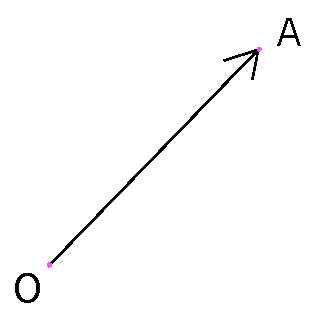
\includegraphics[width=0.8\linewidth]{img/vc-oa.pdf}
%    \caption{ベクトル$\protect \vc{OA} $}%\protectを入れないとなぜかコンパイルが通らない
%     \label{vcoa}
%   \end{minipage}
%   \begin{minipage}[b]{0.45\linewidth}
%     \centering
%     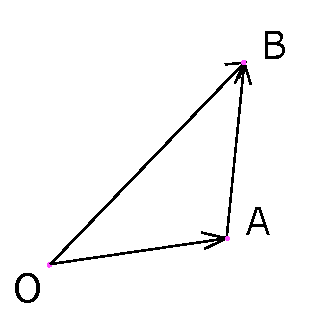
\includegraphics[width=0.8\linewidth]{img/vc-ob.pdf}
%     \caption{ベクトル$\protect \vc{OB}=\protect \vc{OA}+\protect  \vc{AB}$}
%     \label{vcob}
%   \end{minipage}
% \end{figure}


% \begin{figure}[H]
%   \begin{tikzpicture}
%   \draw[->](0,0)--(4,2);
%   \draw(0,0)node[left]{O};
%   \draw(4,2)node[above]{A};
%   \end{tikzpicture}
%   \caption{ベクトル$\protect \vc{OA} $}
% \end{figure}
% \begin{figure}[H]
%   \begin{tikzpicture}
%   \draw[->](0,0)--(2,1);
%   \draw[->](2,1)--(4,3);
%   \draw(0,0)node[left]{O};
%   \draw(2,1)node[above]{A};
%   \draw(4,3)node[above]{B}
%   \end{tikzpicture}
%   \caption{ベクトル$\protect \vc{OB}=\protect \vc{OA}+\protect  \vc{AB}$}
% \end{figure}

\begin{figure}[H]
  \centering
      \begin{tabular}{cc}  
        \begin{minipage}[t]{0.3\linewidth}
          \centering
        \begin{tikzpicture}
          \coordinate (O) at (0,0) node [left] at (O) {O};
          \coordinate (A) at (3,3) node [above] at (A) {A};
      \draw[->](O)--(A);
        \end{tikzpicture}
  \caption{ベクトル$\protect \vc{OA} $}
        \end{minipage} &
        \begin{minipage}[t]{0.3\linewidth}
          \centering
  \begin{tikzpicture}
    \coordinate (O) at (0,0) node [left] at (O) {O};
    \coordinate (A) at (3,1) node [right] at (A) {A};
    \coordinate (B) at (4,3) node [above] at (B) {B};
     \draw[->](O)--(A);
     \draw[->](A)--(B);
     \draw[->](O)--(B);
   \end{tikzpicture}
   \caption{ベクトル$\protect \vc{OB}=\protect \vc{OA}+\protect  \vc{AB}$}
        \end{minipage}
      \end{tabular}
  \end{figure}


また、ここでは特に{\bf 数を並べたもの}と考えることも多い。この2つの表現は当然同じである。
$n$成分をもつベクトル$\vec{v}$は
\begin{equation}
  \vec{v}=\left( \begin{matrix}
    v_{1}\\
    \vdots\\
    v_{n}
  \end{matrix} \right) 
\end{equation}
のように表される。前者の表現のほうが以下に用意する言葉のイメージは付きやすいかもしれない。
向きを持たない量は{\bf スカラー}という。ベクトル$\vec{v}$の大きさを{\bf 絶対値}あるいは{\bf ノルム}と呼び
\begin{equation}
  |\vec{v}| ,\quad \text{あるいは単に細字で}\quad v 
\end{equation}
と書く。$||v||$と2本線で囲むことも多い。数学書ではだいたいこう書かれる。大きさは向きを持たないのでスカラーである。大きさが同じで、向きが全く逆方向のベクトルを逆ベクトルと呼び
\begin{equation}
  -\vec{v}
\end{equation}
と負号を添えて書く。2つのベクトル$\vec{v},\, \vec{w}$の大きさと向きがどちらも同じとき、これらのベクトルは{\bf 等しい}といって
\begin{equation}
  \vec{v} = \vec{w}
\end{equation}
と表す。これは両方のベクトルの各成分が等しいことを意味する。
構成する数が同じであったとしても順番が違えば違うベクトルである。
\begin{equation}
  \left( \begin{matrix}
    1\\
    2\\
    3
  \end{matrix} \right) \neq\left( \begin{matrix}
    1\\
    3\\
    2
  \end{matrix} \right)
\end{equation}
大きさが1のベクトルを{\bf 単位ベクトル}と呼ぶ。例えば$\vec{v}$の方向の単位ベクトルは
\begin{equation}
  e_{\vec{v}}=\frac{\vec{v}}{|v|}
\end{equation}
と表せる。これのことは方向ベクトルとも呼ぶ。なお、方向を指定しないで単位ベクトルと言っても意味がないので注意。
大きさが0のベクトル、すなわち全ての成分が0であるベクトルは{\bf ゼロベクトル}と呼ばれ、$\vec{0}$で表される。単に$0$と表すこともある。
\begin{equation}
  \vec{0}=\left( \begin{matrix}
    0\\
    0\\
    \vdots \\
    0
  \end{matrix} \right)
\end{equation}
また、空間中の点も数を並べて表現されていたので、この点を{\bf 位置ベクトル}という言葉で表せる。例えば3次元空間上の点について
\begin{equation}
    (x,y,z) \quad \leftrightarrow \quad \left( \begin{matrix}
      x\\
      y\\
      z
    \end{matrix} \right)
\end{equation}
で表すことができる。
\subsubsection{演算}
スカラー倍と2つのベクトルの和、内積を定義する。商は定義されない。
成分の数が違うときは和や積を定義できないことに注意。
なお、単に積ではなく内積という言葉を用いたのは外積と呼ばれる積もあるためである。
外積はあとでやるかも。
\begin{framed}
\begin{description}
  \item[スカラー倍] あるベクトル$\vec{v}$をスカラー$a$倍したとき、各成分が$a$倍される。
  \begin{equation}
    a\vec{v}=\left( \begin{matrix}
      av_{1}\\
      \vdots \\
      av_{n}
    \end{matrix} \right)
  \end{equation}
  図的な表現をすれば$a>0$ならば向きは同じで大きさが$|a|$倍され、$a<0$ならば向きは反対で大きさが$|a|$倍されたベクトルとなる。
  \item[和] 2つのベクトルの和は各成分ごとに和を取るものとする。例えば
  \begin{equation}
    \left( \begin{matrix}
      a\\
      b\\
      c
    \end{matrix} \right)+\left( \begin{matrix}
      d\\
      e\\
      f
    \end{matrix} \right)=\left( \begin{matrix}
      a+d\\
      b+e\\
      c+f
    \end{matrix} \right)
  \end{equation}
  である。先に少し述べたような図の描像では、始点から途中の点を介して終点まで向かうように描かれ、最終的には単に始点から終点へ向かうベクトルとなる。
  なお、差については$(-1)$倍して足したと考えるとよい。
  \begin{equation}
    -\vec{v}=(-1)\vec{v}
  \end{equation}
  先に紹介した逆ベクトルとは足したらゼロベクトルになるベクトルとして定義される。
  ゼロベクトルは足しても引いてももとのベクトルは変わらない
  。\footnote{群論の言葉では演算してももとの形のままとなる元を単位元、足して単位元となる元を逆元と呼ぶ。ここでは単位ベクトルとの言葉遣いが紛らわしいのであまり使わないようにする。}
  \item[内積] ベクトル特有の演算である。これは2つのベクトルからスカラーを作り出すものである。$\vec{v},\vec{w}$を$n$成分のベクトルとすると
  \begin{equation}
  \label{in-prod}  \vec{v}\cdot \vec{w} = v_{1}w_{1}+\cdots + v_{n}w_{n}=\sum_{i=1}^{n}v_{i}w_{i}
  \end{equation}
と定義される。内積を$(\vec{v},\vec{w})$や$\braket{\vec{v},\vec{w}}$で表すこともある。ベクトルのノルムはこの内積を用いて定義され、
\begin{equation}
  |\vec{v}|=\sqrt{\vec{v}\cdot \vec{v}}
\end{equation}
である。また、2つのベクトルのなす角$\theta$とすると
\begin{equation}
  \vec{v}\cdot \vec{w}=|\vec{v}||\vec{w}|\cos{\theta}
\end{equation}
と書ける。この書き方についてはきちんと図的な表し方から納得できることを確認してほしい。
\end{description}
\end{framed}
また、以上に関係する諸概念についても紹介する。
\paragraph{距離}ベクトルどうしの距離を定義したい。


まず{\bf 距離}というものを少し堅苦しい書き方ではあるが定義しておく。読み飛ばしても差し支えはない。集合$X$について距離関数
\begin{equation}
  d:X\times X \to \mathbb{R}
\end{equation}
は任意の$X$の元$x,y,z$について以下の条件を満たす。
\begin{enumerate}
  \item $d(x,y)\geq 0$(非負性)
  \item $d(x,y)=d(y,x)$(対称律)
  \item $x=y$のときのみ$d(x,y)=0$
  \item $d(x,y)\leq d(x,z)+d(z,y)$(三角不等式\footnote{劣加法性とも言う。})
\end{enumerate}
ここでは、ベクトルどうしの距離の定義として{\bf Euclid距離}を用いる。すなわち、$\vc{v},\vc{w}$に対して
\begin{equation}
  \label{kyori}d(\vc{v},\vc{w})=\sqrt{|v_{1}-w_{1}|^{2}+\cdots +|v_{n}-w_{n}|^{2}}
\end{equation}
位置ベクトルの考え方を思い出せば、これは単に2点間の距離を表しているにすぎないことがわかる。
三平方の定理の$n$次元への一般化である。
このように定義した距離が上の条件$1.\sim 4.$を満たすことを確認しておこう。
\paragraph{コサイン類似度}
2つのベクトルがどれだけ''近いか''を図る尺度として{\bf コサイン類似度}を定義できる。ベクトル$\vc{v},\vc{w}$に対してコサイン類似度$\mathrm{sim}(\vc{v},\vc{w})$を
\begin{equation}
\label{cossim} \mathrm{sim}(\vc{v},\vc{w})=\frac{\vc{v}\cdot \vc{w}}{|\vc{v}||\vc{w}|}=\cos{\theta}
\end{equation}
によって定める。これは$-1\leq \mathrm{sim}(\vc{v},\vc{w})\leq 1$で''近さ''を判定するものである。例えば$\mathrm{sim}(\vc{v},\vc{w})=1$であれば$\cos{\theta}=1$、すなわち$\theta=0$なので全く同じ方向を向いていて、コサイン類似度の観点からは最も''近い''といえる。
反対に、$\mathrm{sim}(\vc{v},\vc{w})=-1$であれば$\cos{\theta}=-1$、すなわち$\theta=\pi$であるから、全く逆方向に向いているベクトルである。
このとき最も''遠い''と思えるだろう。
なお、定義から分かる通り、コサイン類似度はベクトルの大きさは関係なく、角度で近さを測っている。
\subsubsection{位置ベクトル}
ベクトルと座標の関係をもう少し詳しく説明する。
もともとベクトル自体は座標系によらない量\footnote{直交座標を使おうが極座標を使おうがその矢印そのものは全く変わらずそこに''在る''ため。}であるが、座標を指定すると計算において便利である。


$xy$平面上で図\ref{Aab}のようにA$(a,b)$という点があったとする。
この数字の意味するところはもちろん、「$x$軸方向に$a$だけ進み、$y$軸方向に$b$だけ進んだところ」と解釈する。そして、ベクトル$\vc{OA}$を位置ベクトルとして、点Aを表すものと考える。
\begin{equation}
  A(a,b)\quad\leftrightarrow\quad \vc{OA}=\left(\begin{matrix}
    a\\
    b
  \end{matrix}\right)
\end{equation}
「$x$軸方向に$a$だけ進み、$y$軸方向に$b$だけ進んだところ」を上のように$\vc{OA}$で表せるが、この文言に従えば、もう少し違った表し方があるようにも思える。
「$x$軸、$y$軸方向にそれぞれ基本となるベクトルがあって、それらを何倍かして足し合わせたもの」と表したらどうだろうか。
\begin{equation}
  \vec{e}_{x}=\left(\begin{matrix}
    1\\
    0
  \end{matrix}\right)\quad \vec{e}_{y}=\left(\begin{matrix}
    0\\
    1
  \end{matrix}\right)
\end{equation}
\begin{figure}[H]
  \centering
  \begin{tabular}{cc}  
    \begin{minipage}[t]{0.3\linewidth}
      \centering
      \begin{tikzpicture}
        \node (O) at (-0.5,-0.5) {O};%原点
       \coordinate (A) at (2,1);
       \coordinate (Ax) at (2,0)node [below] at (Ax) {$a$};
       \coordinate (Ay) at (0,1)node [left] at (Ay) {$b$};
       \coordinate (x) at (3,0)node [right] at (x) {$x$};
       \coordinate (y) at (0,3)node [right] at (y) {$y$};

        \fill (A)circle(1pt) node[above]{A};
        \draw[->](-1,0)--(3,0);%x軸
        \draw[->](0,-1)--(0,3);%y軸
        \draw[dotted](Ax)--(A);
        \draw[dotted](Ay)--(A);
        \draw[->](0,0)--(A);
      \end{tikzpicture}
\caption{点A$(a,b)$}
\label{Aab}
    \end{minipage} &
    \begin{minipage}[t]{0.3\linewidth}
      \centering      \begin{tikzpicture}
        \node (O) at (-0.5,-0.5) {O};%原点
       \coordinate (A) at (2,1);
       \coordinate (Ax) at (2,0)node [below] at (Ax) {$a$};
       \coordinate (Ay) at (0,1)node [left] at (Ay) {$b$};
       \coordinate (x) at (3,0)node [right] at (x) {$x$};
       \coordinate (y) at (0,3)node [right] at (y) {$y$};

        \fill (A)circle(1pt) node[above]{A};
        \draw[->](-1,0)--(3,0);%x軸
        \draw[->](0,-1)--(0,3);%y軸
        \draw[dotted](Ax)--(A);
        \draw[dotted](Ay)--(A);
        \draw[red,->](0,0)--(0.5,0) node [below] {$\vec{e}_{x}$};
        \draw[blue,->](0,0)--(0,0.5)node [left] {$\vec{e}_{y}$};
      \end{tikzpicture}
\caption{点A$(a,b)$}
    \end{minipage}
  \end{tabular}
\end{figure}

この基本となるベクトルのことをそのまま{\bf 基本ベクトル}、または{\bf 基底ベクトル}と呼ぶ。
線形代数の文脈では基底ベクトルと呼ぶことのほうが多い。
\begin{equation}
 \vc{OA}=\left(\begin{matrix}
    a\\
    b
  \end{matrix}\right)=a
  \underbrace{ \left(\begin{matrix}
    1\\
    0
  \end{matrix}\right)}_{\text{$x$方向}}
+b\underbrace{\left(\begin{matrix}
    0\\
    1
  \end{matrix}\right)}_{\text{$y$方向}}
\end{equation}
基底ベクトルはよく$\vec{e}$で表される。詳しいことは後の項で記すが、この基底ベクトルのように
\begin{equation}
  c_{x}\vec{e}_{x}+c_{y}\vec{e}_{y}=0
\end{equation}
を満たすような係数$c$が$c_{x}=c_{y}=0$のみであるとき、{\bf 1次独立}であるという。また、このようないくつかのベクトルをスカラー倍して和を取ったものを{\bf 1次結合}という。
この例から、2次元平面上では1次独立なベクトルが2つあればそれらの1次結合によってどんなベクトルも表すことができるということが理解できるとよい。

\subsection{具体例}
ここまでの内容を用いてできる具体例を記す。ここでは、距離とコサイン類似度を用いた類似性の判定についてである。
\subsubsection{色の比較}
もっとも簡単に{\bf 色}を表す方法は{\bf RGB}だろう。これは赤、緑、青の三原色を用いて一つの色を表す方法である。
よって、色は{\bf 3成分のベクトル}で表されるものとなる。上での例では成分は2つだったが、3つに増えても同じである。
ここでは各成分が0から255までの値で表されるものとする。


ここでの問題設定は「オレンジ色は赤色、黄色、青色のどの色に最も近いか」としよう。
オレンジ色、赤色、黄色、青色のベクトルをそれぞれ$\vec{o},\vec{r},\vec{y},\vec{b}$とおくと、次のように表せる。
\begin{equation}
  \vec{o}=\left( \begin{matrix}
    255\\
    165\\
    0
  \end{matrix}\right),\quad 
  \vec{r}=\left( \begin{matrix}
    255\\
    0\\
    0
  \end{matrix}\right),\quad 
  \vec{y}=\left( \begin{matrix}
    255\\
    255\\
    0
  \end{matrix}\right),\quad 
  \vec{b}=\left( \begin{matrix}
    0\\
    0\\
    255
  \end{matrix}\right),\quad 
\end{equation}


まず距離を使って比較してみる。それぞれ(\ref{kyori})を用いて計算すると
\begin{align}
  d(\vec{o},\vec{r})&=\sqrt{|255-255|^{2}+|165-0|^{2}+|0-0|^{2}}=165\\
  d(\vec{o},\vec{y})&=\sqrt{|255-255|^{2}+|165-255|^{2}+|0-0|^{2}}=90\\
  d(\vec{o},\vec{b})&=\sqrt{|255-0|^{2}+|165-0|^{2}+|0-255|^{2}}\approx 396.6
\end{align}
となる。これはそのままどれだけ離れているかを表しているので、オレンジ色には黄色、赤色、青色の順で似ているといえる。


次にコサイン類似度を用いてみる。角度で近さを考えるので、ベクトルのなす角が0、すなわち値が1に近いほど似ていて、なす角が$\pi$、すなわち値が$-1$に近いほど似ていないということになる。(\ref{cossim})を用いてやれば
\begin{align}
  \mathrm{sim}(\vec{o},\vec{r})&=\frac{255\times 255 +165\times 0 +0\times0}{\sqrt{|255|^{2}+|165|^{2}+|0|^2}\sqrt{|255|^{2}+|0|^{2}+|0|^2}}\approx 0.84\\
  \mathrm{sim}(\vec{o},\vec{y})&=\frac{255\times 255 +165\times 255 +0\times0}{\sqrt{|255|^{2}+|165|^{2}+|0|^2}\sqrt{|255|^{2}+|255|^{2}+|0|^2}}\approx 0.98\\
  \mathrm{sim}(\vec{o},\vec{b})&=\frac{255\times 0 +165\times 0 +0\times255}{\sqrt{|255|^{2}+|165|^{2}+|0|^2}\sqrt{||^{2}+|0|^{2}+|255|^2}}= 0
\end{align}
これもまた、黄色、赤色、青色の順で似ているという結果になった。

これを応用すれば、画像データから色を抽出してベクトルにして画像同士の似ている・似ていないを定量的に計算できるだろう\footnote{やってないけど。}。
\subsubsection{Bag of Words}
コサイン類似度は文章の近さについても使える。
文章をベクトルにするとき{\bf Bag of Words}という手法を使う。例えば以下の3つの文章を考える。
\begin{enumerate}
  \item :「私はラーメンと餃子が好きです」
  \item :「私は餃子が嫌いです」
  \item :「私はラーメンが好きです」
\end{enumerate}
上の文章に出てくる自立語は「私」「ラーメン」「餃子」「好き」「嫌い」である。つまり、これらの自立語の有無によって文章を特徴づける。
この''特徴づけ''をベクトルにするため、5成分のベクトルとして、順にその言葉が出たら1を、出なければ0をその値とする。
文章のベクトルをそれぞれ$\vec{A},\vec{B},\vec{C}$で表せば
\begin{equation}
  \vec{A}=\left( \begin{matrix}
    1\\
    1\\
    1\\
    1\\
    0
  \end{matrix}\right),\quad ,\vec{B}=\left( \begin{matrix}
    1\\
    0\\
    1\\
    0\\
    1
  \end{matrix}\right),\quad \vec{C}=\left( \begin{matrix}
    1\\
    1\\
    0\\
    1\\
    0
  \end{matrix}\right)
\end{equation}
と書ける。このように用意すればsimを用いて近さを測ることができる。
この方法でベクトルにしたとき、距離の使用は類似性の判定に向かない。
なぜならば文章が長いほど多くの成分が1になり、また短ければ多くの成分が0となるためである。
すなわち、長い文章と短い文章を比較したときには内容にかかわらず距離が大きく出てしまうのである。

\section{行列}
新たに出てくる言葉や概念が多いので注意深く見ていく。
\subsection{基本事項}
行列について、ゼロ行列、正方行列、単位行列、対角行列、スカラー行列、上三角行列、下三角行列、転置、対称行列、反対称行列(交代行列)。行ベクトル、列ベクトル。添字。
\subsubsection{行列}
横と縦に長方形に数を並べたものを{\bf 行列}という。並べられた数をそれぞれ{\bf 成分}といい、数は$(\,)$や$[\,]$で囲む。
横に並んだ成分を{\bf 行}、縦に並んだ成分を{\bf 列}という。
例えば3行4列の行列であるとすれば成分を$a_{ij}(i=1,2,3,\, j=1,2,3,4)$のように表して
\begin{equation}\left(
 \begin{matrix}
    a_{11} & a_{12} & a_{13} & a_{14} \\
    a_{21} & a_{22} & a_{23} & a_{24} \\
    a_{31} & a_{32} & a_{33} & a_{34} 
  \end{matrix}\right) \quad , \quad \left[
    \begin{matrix}
      a_{11} & a_{12} & a_{13} & a_{14} \\
      a_{21} & a_{22} & a_{23} & a_{24} \\
      a_{31} & a_{32} & a_{33} & a_{34} 
    \end{matrix}\right]
\end{equation}
である。一般に$m$行$n$列である行列は$m\times n$行列や$(m,n)$型の行列などという。この行と列の組$(m,n)$を行列の{\bf 型}や{\bf サイズ}という。
\begin{equation}
  \label{gyoretu}  A=
  \left(
 \begin{matrix}
    a_{11} & \cdots & a_{12} & \cdots & a_{1n} \\
    \vdots &        & \vdots &        & \vdots \\
    a_{i1} & \cdots & a_{ij} & \cdots & a_{in}\\ 
    \vdots &        & \vdots &        & \vdots \\
    a_{m1} & \cdots & a_{mj} & \cdots & a_{mn} 
  \end{matrix}\right)
\end{equation}
このうち 
\begin{equation}
  a_{ij} , \quad (a_{i1} \quad a_{i2} \quad \cdots \quad a_{in} ),\quad  \left( \begin{matrix}
    a_{1j}\\
    a_{2j}\\
    \vdots\\
    a_{mj}
  \end{matrix}\right)
\end{equation}
の部分をそれぞれ行列$A$の$(i,j)$成分、第$i$行、第$j$列という。
上の表し方で$a_{ij}$の$ij$を{\bf 添字}という。\footnote{単に変数や文字を簡潔に表す記法である。しかしこの添字記法は計算を便利にし、Einstein規約によって様々な計算が一気に簡単になる。なお、下付きの添字以外に上付き添字を使うこともあるので添字の記法を見たときは十分に注意すること。}
この添字は必ず行・列の順になっていることに注意。
$m\times n$行列$A$の成分を$a_{ij}$と書いたとき
\begin{equation}
  A=(a_{ij})_{m\times n}
\end{equation}
と略記することもある。なお、行列の型が明らかなときは${}_{m\times n}$を省略することもある。
以下にいくつか行列に関する言葉を用意する。多いので少しずつ覚えてほしい。また、添字の記法を多用しているのでこれも慣れていくことをおすすめする。
\begin{framed}
\begin{description}
  \item[$1\times 1$行列] $(a)$のように表されるがこの場合普通の数$a$と同一視して単に$a$と表す。
  \item[行列の相等] 2つの行列$A$と$B$が{\bf 等しい}とは、それぞれの型が同じで、対応する成分がそれぞれすべて等しいことを意味する。すなわち、$A=(a_{ij})_{m\times n}$と$B=(b_{kl})_{p\times q}$において$m=p$かつ$n=q$で、任意の$i,j$において$a_{ij}=b_{ij}$が成り立つとき、
  \begin{equation}
    A=B
  \end{equation}
  である。等しくないときは
  \begin{equation}
  A\neq B 
  \end{equation}
  と書かれる。もちろんベクトルと同じようにどれか一つの成分でも違えば$A\neq B$である。
  \item[ゼロ行列] すべての成分が0である$m\times n$行列を{\bf ゼロ行列}といい、$O_{m,n}$や$O$と書く。
  例えば$3\times 2$のゼロ行列は
  \begin{equation}\left( 
    \begin{matrix}
      0 & 0\\
      0 & 0\\
      0 & 0
    \end{matrix}\right) 
  \end{equation}
  のようになる。
  \item[正方行列] 行列$A$の行と列の数が同じとき、すなわち$n\times n$行列のときAを$n$次の{\bf 正方行列}、または$n$次行列という。
 $A=(a_{ij})_{n\times n}$のうち成分$a_{11},a_{22},\cdots,a_{nn}$を$A$の{\bf 対角成分}という。
  例えば2次正方行列は
   \begin{equation}
  A=\left( 
\begin{matrix}
  a & b \\
  c & d
\end{matrix}
  \right)  
  \end{equation}
  のように書けて、対角成分は$a,d$である。文字通り対角線の成分のことである。
  \item[対角行列] 正方行列$A$が対角成分以外を持たない、すなわち$i\neq j$のとき
  \begin{equation}
  a_{ij}=0  
  \end{equation}
  である行列を{\bf 対角行列}という。
  \begin{equation}
    \left( \begin{matrix}
      a_{11} & 0 & \cdots & 0 \\
      0 & a_{22} & \cdots & 0 \\
      \vdots  & \vdots  & \ddots & \vdots \\
      0& 0 & \cdots & a_{nn}
    \end{matrix} \right)
  \end{equation}
  \item[スカラー行列] 対角行列のうち、すべての対角成分が等しい行列、すなわち
\begin{equation}
  a_{ij} =\begin{cases}
    0 & (i\neq j)\\
    a& (i=j)
  \end{cases}
\end{equation}
  のとき{\bf スカラー行列}という。
  \begin{equation}
    \left( \begin{matrix}
      a & 0 & \cdots & 0 \\
      0 & a & \cdots & 0 \\
      \vdots  & \vdots  & \ddots & \vdots \\
      0& 0 & \cdots & a
    \end{matrix} \right)
  \end{equation}
  \item[単位行列] スカラー行列のうちすべての対角成分が1である、すなわち
  \begin{equation}
    a_{ij}=\begin{cases}
      0 & (i\neq j)\\
      1& (i=j)
    \end{cases}
  \end{equation}
  のとき{\bf 単位行列}といい、$n\times n$行列であれば$n$次単位行列といい$I_{n}$や$E_{n}$、あるいは単に$I$や$E$と書く。
  \begin{equation}
   I_{n} = \left( \begin{matrix}
      1 & 0 & \cdots & 0 \\
      0 & 1 & \cdots & 0 \\
      \vdots  & \vdots  & \ddots & \vdots \\
      0& 0 & \cdots & 1
    \end{matrix} \right)
  \end{equation}
  なお、以下のように$i=j$のときは1、それ以外は0となる記号として{\bf Kroneckerのデルタ}を定義すると便利である。
  \begin{equation}
    \delta_{ij}=\begin{cases}
      0 & (i\neq j)\\
      1& (i=j)
    \end{cases}
  \end{equation}
  これを用いればスカラー行列や単位行列をそれぞれ
  \begin{equation}
    A=(a\delta_{ij})_{n\times n},\quad I_{n}=(\delta_{ij})_{n\times n}
  \end{equation}
  と表せる。
  \item[三角行列] 正方行列$A=(a_{ij})_{n\times n}$について
  \begin{equation}
    a_{ij}=0 \quad (i>j)
  \end{equation}
  のとき{\bf 上三角行列}といい、
  \begin{equation}
    a_{ij}=0 \quad (i<j)
  \end{equation}
  のとき{\bf 下三角行列}という。3次行列でそれぞれの例を書けば、
  \begin{equation}
    \left( 
      \begin{matrix}
        1 & 2 & 3 \\
        0 & 4 & 5  \\
        0 & 0 & 6  \\
      \end{matrix}
    \right) \quad , \quad\left( 
      \begin{matrix}
        1 & 0 & 0 \\
        2 & 4 & 0  \\
        3 & 5 & 6  \\
      \end{matrix}
    \right)
  \end{equation}
  \item[転置行列] $m\times n$行列$A$の行と列を入れ替えて得られる$n\times m$行列を$A$の転置行列といい、${}^{t}A$とかく。\footnote{他に$A^{t},{}^{T}A,A^{T}$などと書くこともある。物理の文脈では一番最後の記法が多い。}例えば
    \begin{equation}
      \left( 
        \begin{matrix}
          1 & 2 & 3 \\
          4 & 5 & 6 
        \end{matrix}
      \right) \quad \overset{転置!}{\to} \quad\left( 
        \begin{matrix}
          1 & 4  \\
          2 & 5   \\
          3 & 6 
        \end{matrix}
      \right)
    \end{equation}
    転置行列を求めることを、「転置を取る」と表現する。
  \item[対称行列] もとの行列と転置行列が一致するとき、その行列を対称行列という。例えば
  \begin{equation}
 \label{taisho}   \kakko{ \, 1 \, }\quad \left( 
      \begin{matrix}
        1 & 2  \\
        2 & 4  
      \end{matrix}
    \right) \quad \left( 
      \begin{matrix}
        1 & 2 & 3 \\
        2 & 5 & 6 \\
        3 & 6 & 0
      \end{matrix}
    \right)
  \end{equation}
  なお、$n$次正方行列$A=(a_{ij})$が対称行列であるときの必要十分条件は
  \begin{equation}
    a_{ij}=a_{ji}
  \end{equation}
  である。
\end{description}
\end{framed}
以上で一気に言葉を定義したので、おそらくすぐに慣れることは難しいだろう。例題を少し用意したので少し手を動かしてやってみてほしい。
\begin{description}
  \item[例3.1] 次の行列の型、$(1,2)$成分、第2行、第3列をそれぞれ答えよ。
  \begin{equation}
    \left( 
      \begin{matrix}
        1 & 2 & 4 \\
        7 & 3 & 6
      \end{matrix}
    \right)
  \end{equation}
  \item[例3.2] 次の正方行列の型を答えよ。また、対角成分をすべて書き出し、足しあわせよ。
  \begin{equation}
  \label{rei32}  \left( 
      \begin{matrix}
        2 & 6 & 9 & 8\\
        0 & 2 & 7 & 0 \\
        3 & 6 & 9 & 9 \\
        8 & 1 & 7 & 0
      \end{matrix}
    \right)
  \end{equation}
  \item[例3.3] 2次単位行列を具体的に書いてみよ。
  \item[例3.4] $(i,j)$成分が$2\delta_{ij}$で表される3次行列を具体的に書き表せ。 
  \item[例3.5] $(i,j)$成分が$2\delta_{i\, j+1}$で表される3次行列を具体的に書き表せ。 
  \item[例3.6] (\ref{rei32})の転置行列を書け。
  \item[例3.7] 実際に(\ref{taisho})の転置を取って元の行列と一致するか確かめよ。
\end{description}
なお、$1\times n$行列を$n$次の{\bf 行ベクトル}、$m\times 1$行列を$m$次の{\bf 列ベクトル}といい、行ベクトルと列ベクトルをあわせて{\bf 数ベクトル}という。
例えば3次の行ベクトルは
\begin{equation}
  (\, a \quad b \quad c \,)
\end{equation}
3次の列ベクトルは
\begin{equation}
  \kakko{
    \begin{matrix}
      a\\
      b\\
      c
    \end{matrix}
  }
\end{equation}
などのようになる。


%演算の定義、和・スカラー倍の交換律、結合律、分配律。積の非可換性。いちおう逆行列。
\subsubsection{和とスカラー倍}
さて、行列に関する演算を定義していく。まず{\bf 和}について考える。
ともに$n\times m$行列である$A$と$B$に対して和を、{\bf 各成分同士を足すこと}と定義する。型が違う行列については演算が定義できないことに注意せよ。
添字を用いて書き表わせば
\begin{equation}
  A=(a_{ij})_{n\times m},\quad B=(b_{ij})_{n\times m}
\end{equation}
に対して和$A+B$を
\begin{equation}
  (A+B)_{n\times m}=(a_{ij}+b_{ij})_{n\times m}
\end{equation}
と定義する。例えば$2\times 3$行列の和は
\begin{equation}
  \left( 
    \begin{matrix}
      a & b & c \\
      d & e & f
    \end{matrix}
  \right)
+
\left( 
  \begin{matrix}
    g & h & i \\
    j & k & l
  \end{matrix}
\right)=\left( 
  \begin{matrix}
    a+g & b+h & c+i \\
    d+j & e+k & f+l
  \end{matrix}
\right)
\end{equation}
と書かれる。\\
次に{\bf スカラー倍}を定義する。
スカラー、すなわち大きさのみを持つ数\footnote{単に実数や複素数と思えばよい。}$c$に対して、$n\times m$行列$A$の$c$によるスカラー倍とは、{\bf すべての成分を$c$倍するもの}と定義する。
ここでも添字を用いて表せば
\begin{equation}
  cA = (ca_{ij})_{n\times m}
\end{equation}
である。
例えば次の$2\times 3$行列を$c$倍すると
\begin{equation}
  c \left( 
       \begin{matrix}
        1 & 2 & 4 \\
        7 & 3 & 6
      \end{matrix}
    \right)
    =
    \left( 
      \begin{matrix}
        c & 2c & 4c \\
        7c & 3c & 6c
      \end{matrix}
    \right)
\end{equation}
となる。
例題として次の計算をせよ。
\begin{description}
  \item[例3.8] 
  \begin{equation}
    \left(  
      \begin{matrix}
        1 & 2 & 4 \\
        7 & 3 & 6
      \end{matrix}
    \right)+\left(  
      \begin{matrix}
        3 & 2 & 1 \\
        5 & 6 & 7
      \end{matrix}
    \right)
  \end{equation}
  \item[例3.9] 
  \begin{equation}
   3 \left( 
      \begin{matrix}
        2 & 6 & 9 \\
        0 & 2 & 7  \\
        3 & 6 & 9 
      \end{matrix}
    \right)
  \end{equation}
  \item[例3.10] \begin{equation}
    \left(  
      \begin{matrix}
        1 & 2  \\
        2 & -3 
      \end{matrix}
    \right)+ 2 \left(  
      \begin{matrix}
        3 & 1 \\
        -1 & 1 
      \end{matrix}
    \right)
  \end{equation}
\end{description}
ここで$(-1)$倍について述べておく。
便利な記法として
\begin{equation}
  (-1)A=-A
\end{equation}
と書く。また、
\begin{equation}
  A+(-B)=A-B
\end{equation}
と書くことに注意せよ。
和とスカラー倍について以下の定理が成り立つ。これは後に扱うベクトル空間が満たすべき基本的性質である。
\begin{screen}
  \begin{thm}[和とスカラー倍]
  $m\times n$行列$A,\, B,\, C$またゼロ行列$O_{m,n}$とスカラー$c, \, d$に対して、以下の$(\mathrm{A})\sim (\mathrm{H})$が成り立つ。
  \begin{enumerate}
    \item  $A+B=B+A\quad $(和の交換律)
    \item  $(A+B)+C=A+(B+C)\quad $(和の結合律)
    \item $A+O_{m,n}=O_{m,n}+A=A$
    \item $c(dA)=(cd)A\quad $(スカラー倍の結合律)
    \item $(c+d)A=cA+dA \quad $(分配律I)
    \item $c(A+B)=cA+cB \quad $(分配律II)
    \item $1A=A$
    \item $0A=O_{m,n}$
  \end{enumerate}
  \end{thm}
\end{screen}
なお和の結合律により$(A+B)+C=A+(B+C)=A+B+C$と書いてよい。
この項の最後に、対称行列と対になる概念として{\bf 交代行列}を定義する。
\begin{framed}
\begin{description}
  \item[交代行列] ${}^{t}A=-A$となる正方行列$A$を{\bf 交代行列}、あるいは{\bf 反対称行列}という。
\end{description}
\end{framed}
例えば
\begin{equation}
  \left(  
      \begin{matrix}
        0 & 2  \\
        -2 & 0
      \end{matrix}
    \right), \quad \left(  
      \begin{matrix}
        0 & 1 & 2\\
        -1 & 0 & 3\\
        -2& -3 & 0 
      \end{matrix}
    \right)
\end{equation}
などである。
\begin{screen}
  \begin{thm}
    $n$次正方行列$A=(a_{ij})_{n\times n}$が交代行列であるための必要十分条件は
    \begin{equation}
  \label{kotai}    a_{ij}=-a_{ji} \quad (i,j=1,2,\cdots ,n)
    \end{equation}
    であり、交代行列の対角成分はすべて0である。
  \end{thm}
\end{screen}
この主張を示していく。(\ref{kotai})は定義式${}^{t}A=-A$を成分で表したものであるため、必要十分条件である。
次に対角成分がすべて0であることを示す。
対角成分は$i=j$であるため、(\ref{kotai})と合わせて
\begin{equation}
  a_{ii}=-a_{ii}
\end{equation}
が成り立つ。よって
\begin{equation}
  2a_{ii}=0  \quad  \therefore \, a_{ii}=0
\end{equation}
である。
\subsubsection{積}
$l\times \bm{m}$行列$A=(a_{ij})_{l\times \bm{m}}$と$\bm{m}\times n$行列$B=(b_{jk})_{\bm{m}\times n}$の{\bf 積}$AB$を次のように定義する。
\begin{equation}
  AB=(c_{ik})_{l\times n},\quad c_{ik}=\sum_{j=1}^{m} a_{ij}b_{jk}\quad (i=1,2,\cdots ,l,\, k=1,2,\cdots , n)
\end{equation}
この式の意味は、「行列$AB$の$(i,k)$成分$c_{ik}$が、$A$の行の成分と$B$の列の成分のそれぞれをかけて足したものとなるように定義する」ということである
一般にこの積の順序は可換ではないことに注意。
この節の始めの文章では太字にして強調してあるように、$A$の列の個数と$B$の行の個数が等しいときにのみ積が定義されるので、これを入れ替えると定義できなくなるためである。
%図を入れて説明したい。

\begin{figure}[H]
  
\begin{equation}
  \left( 
   \begin{matrix}
            & \cdots &    & \cdots & \\
          \textcolor{red}{a_{i1}} & \cdots & \textcolor{blue}{a_{ij}}   & \cdots &  \textcolor{green}{a_{im}}  \\
            & \cdots &     & \cdots & 
   \end{matrix}
 \right)    \left( 
  \begin{matrix}
           & \textcolor{red}{b_{1k}} & \\
    \vdots & \vdots & \vdots\\
           & \textcolor{blue}{b_{jk}} & \\
    \vdots & \vdots & \vdots \\
           & \textcolor{green}{b_{mk}} & 
  \end{matrix}
\right)
\end{equation}
  \caption{この行列の積の第$(i,k)$成分は、ここで同じ色をつけたところをかけて足したものとなる。順にかけてすべて足すのである。}
\end{figure}
以下の計算を試してみよ。
計算の結果として型がどうなるかをきちんと注意すること。
\begin{description}
  \item[例3.11] $2$次正方行列どうしの積。これはすべて書いてしまっているが、きちんと計算があっているか確認してほしい。\begin{equation}
    \left( 
     \begin{matrix}
         a & b \\
         c & d
     \end{matrix}
   \right)\left( 
    \begin{matrix}
        e & f \\
        g & h
    \end{matrix}
  \right)=\left( 
    \begin{matrix}
        ae+bg & af+bh \\
        ce+dg & cf+dh
    \end{matrix}
  \right)
  \end{equation}
  \item[例3.12(a)] $2$次正方行列どうしの積。
  \begin{equation}
    \left( 
     \begin{matrix}
         1 & 2 \\
         3 & 4
     \end{matrix}
   \right)\left( 
    \begin{matrix}
        5 & 6 \\
        7 & 8
    \end{matrix}
  \right)
  \end{equation}
  \item[例3.12(b)] $2$次正方行列どうしの積。
  \begin{equation}
    \left( 
    \begin{matrix}
        5 & 6 \\
        7 & 8
    \end{matrix}
  \right)\left( 
    \begin{matrix}
        1 & 2 \\
        3 & 4
    \end{matrix}
  \right)
  \end{equation}
  \item[例3.13] $2\times 3$行列と$3\times 1$行列の積。
  \begin{equation}
    \left( 
     \begin{matrix}
         0 & 1 & 2\\
         1 & 2 & 0
     \end{matrix}
   \right)\left( 
    \begin{matrix}
        3\\
        4\\
        5
    \end{matrix}
  \right)
  \end{equation}
  \item[例3.14] 3次正方行列どうしの積。
  \begin{equation}
    \left( 
     \begin{matrix}
         0 & 1 & 2\\
         1 & 2 & 0\\
         2 & 0 & 1
     \end{matrix}
   \right)\left( 
    \begin{matrix}
        1 & 0 & 0 \\
        0 & 1 & 0 \\
        0 & 0 & 1 \\
    \end{matrix}
  \right)
  \end{equation}
\item[例3.15] $2\times 1$行列と$1\times 2$行列の積。
\begin{equation}
  \left( 
   \begin{matrix}
        1 \\
        2 
   \end{matrix}
 \right)\left( 
  \begin{matrix}
      3 & 4
  \end{matrix}
\right)
\end{equation}
\item[例3.16] $1\times 2$行列と$2\times 1$行列の積。
\begin{equation}
  \left( 
   \begin{matrix}
        1 & 2 
   \end{matrix}
 \right)\left( 
  \begin{matrix}
       3 \\
       4
  \end{matrix}
\right)
\end{equation}

\end{description}
例3.12は積の順序を入れ替えただけである。
前述の通り、積の順序が可換で無いことがわかる。
$n$次正方行列の$A,B$について、積$AB$と$BA$はともに$n$次正方行列となるが、これらが一致するとは限らないのである。
$AB=BA$が成立するとき、この2つの行列$A$と$B$は{\bf 可換}である、または{\bf 交換可能}であるという。
なお、可換でないときは{\bf 非可換}であるという。
例えば、任意の行列$A$に対して、その行列と積の演算が可能な型の単位行列$I$との積は可換である。
例3.14のように行列の形は変わらない。
\begin{equation}
\label{tanni-gyoertu}  AI=IA=A
\end{equation}

また、例3.15,3.16は行ベクトルや列ベクトルの積と見れることに注目してほしい。例3.15は2次正方行列となるが、例3.16は1次正方行列、すなわち通常の数と見なせる。
計算過程を細かく見れば、内積の計算(\ref{in-prod})と同じであることに気づく。
よって$n\times 1$行列としての$n$次列ベクトル$\vc{v},\vc{w}$の{\bf 内積}が次のように表せる。
行列の考えから、前側のベクトルは転置を取って$1\times n$行列である行ベクトルにする。
\begin{equation}
  \vc{v}\cdot\vc{w}={}^{t}\vc{v}\vc{w}=\kakko{v_{1} \quad \cdots \quad v_{n} }
  \kakko{\begin{matrix}
    w_{1}\\
    \vdots \\
    w_{n}
  \end{matrix}
  }=v_{1}w_{1}+\cdots +v_{n}w_{n}
\end{equation}
これ以降、行列の和や積について考えるときは必ず演算が可能な型であるものとする。
\begin{screen}
  \begin{thm}
    $A,B,C$を行列とすると、次の(A)$\sim$(D)が成り立つ。
    \begin{enumerate}
      \item $(AB)C=A(BC)$ (積の結合律) 
      \item $(A+B)C=AC+BC$ (分配律I)
      \item $A(B+C)=AB+AC$ (分配律II)
      \item スカラー$c$に対して$(cA)B=A(cB)=c(AB)$
    \end{enumerate}
  \end{thm}
\end{screen}
なお、積の結合律より$(AB)C=A(BC)=ABC$と括弧を省略して書いてよい。
スカラー行列が$cI$と書けることから、(\ref{tanni-gyoertu})と合わせて考えればスカラー行列をかけることはスカラー倍と同じ意味があることがわかる。

積の結合律より、正方行列にはべき乗、すなわち同じ正方行列を何度もかけることが考えられる。
正方行列$A$に対して、これを$n$回($n=0,1,2,\cdots$)かけたものを$A^{n}$と書いて、$A$の{\bf $n$乗}という。
ただし、$n=0$のとき$A^{0}=I$とする。
通常の数のように以下の{\bf 指数法則}が成り立つ。
\begin{equation}
  A^{n}A^{m}=A^{n+m},\quad (A^{n})^{m}=A^{nm} \quad(n,m=0,1,2,\cdots )
\end{equation}
次の計算をせよ。
\begin{description}
  \item[例3.17] 
  \begin{equation}
  \kakko{\begin{matrix}
    0&1\\
    1&0
  \end{matrix} }^{3}
  \end{equation}
  \item[例3.18]   \begin{equation}\kakko{\begin{matrix}
    0&1\\
    0&0
  \end{matrix}}^{2}
\end{equation}
\end{description}
ここで例3.18を見るとわかるように、通常の数の場合とは違って、ゼロ行列でなくとも何度かかけてゼロ行列になる行列がある。
\begin{framed}
  \begin{description}
    \item[べきゼロ行列] ある自然数$n$に対して$A^{n}=O$となるような行列を{\bf べきゼロ行列}という。
  \end{description}
  \end{framed}
この項の最後に、転置と行列の演算の関係について述べておく。
\begin{screen}
  \begin{thm}
    $A,B$を行列とすると、次の(A)$\sim$(C)が成り立つ。
    \begin{enumerate}
      \item ${}^{t}(A+B)={}^{t}A+{}^{t}B$ 
      \item ${}^{t}(AB)={}^{t}B\,{}^{t}A$
      \item スカラー$c$に対して${}^{t}(cA)=c\,{}^{t}A$
    \end{enumerate}
  \end{thm}
\end{screen}
積の転置を取ると、順序が入れ替わることに注意である。

\subsection{具体例}
以上の積の解説から(\ref{saisho})の例の気持ちが少しだけわかるかもしれない。
しかし、行列の積の利用としてわかりやすいのは図形への応用である。
例えば座標$(x,y)$を何かの変換を施して$(x',y')$にすることは、変換行列$A=(a_{ij})_{2\times 2}$を用いて、点を位置ベクトルで表し、
\begin{equation}
 \label{1ji} \kakko{\begin{matrix}
 a_{11} & a_{12}  \\
 a_{21} & a_{22}
  \end{matrix}}
  \kakko{\begin{matrix}
 x  \\
 y
  \end{matrix}}=
  \kakko{\begin{matrix}
 x'  \\
 y'
  \end{matrix}}
\end{equation}
のように書ける。詳しくは後の章で述べるが、このような行列による変換を線形変換、または1次変換という。
\begin{framed}
  \begin{description}
    \item[恒等変換] 
    単位行列をかけても形は変わらないので、この変換は{\bf 恒等変換}と呼ばれる。
    \begin{equation}
      \kakko{\begin{matrix}
      1 & 0  \\
      0 & 1
      \end{matrix}}
      \kakko{\begin{matrix}
     x  \\
     y
      \end{matrix}}=
      \kakko{\begin{matrix}
     x  \\
     y
      \end{matrix}}
    \end{equation}
  \end{description}
\end{framed}
図形は点の集合であるため、変換をそれぞれの点に施すことで画像の変換処理を行うことができる。(\ref{1ji})は1つの点ついてのみだが、複数の点について同時に変換することもできる。
変換されるベクトルを位置ベクトル$\vc{r}_{i}=(x_{i},y_{i})$を2つ列方向に並べて
\begin{equation}
  X=(\vc{r}_{1}\quad \vc{r}_{2})=
  \kakko{
    \begin{matrix}
      x_{1} & x_{2}\\
      y_{1} & y_{2}
    \end{matrix}
  }
\end{equation}
と行列にすればよい。実際に$AX$がそれぞれの点$\vc{r}_{i}$を変換していることを確かめよ。
\subsubsection{拡大・縮小}
まず、図形を$2$倍に拡大することを考える。つまり、点の位置を原点に対して$2$倍離れた場所に移動させればよい。
例えば、$(2,1)\to (4,2)$としたい。
\begin{equation}
  \kakko{ 
    \begin{matrix}
      2\\
      1
    \end{matrix}
  } \to 
    \kakko{ 
      \begin{matrix}
        4\\
        2
      \end{matrix}
    } 
\end{equation}

\begin{figure}[H]
  \centering
  \begin{tabular}{cc}  
    \begin{minipage}[t]{0.3\linewidth}
      \centering
      \begin{tikzpicture}
        \node (O) at (-0.5,-0.5) {O};%原点
       \coordinate (A) at (2,1);
       \coordinate (Ax) at (2,0)node [below] at (Ax) {$2$};
       \coordinate (Ay) at (0,1)node [left] at (Ay) {$1$};
       \coordinate (x) at (3,0)node [right] at (x) {$x$};
       \coordinate (y) at (0,3)node [right] at (y) {$y$};

        \fill (A)circle(1pt) node[above]{A};
        \draw[->](-1,0)--(3,0);%x軸
        \draw[->](0,-1)--(0,3);%y軸
        \draw[dotted](Ax)--(A);
        \draw[dotted](Ay)--(A);
        \draw[->](0,0)--(A);
      \end{tikzpicture}
\caption{点A$(2,1)$}
\label{kakudai}
    \end{minipage} &
    \begin{minipage}[t]{0.3\linewidth}
      \centering      \begin{tikzpicture}
        \node (O) at (-0.5,-0.5) {O};%原点
       \coordinate (A) at (4,2);
       \coordinate (Ax) at (4,0)node [below] at (Ax) {$4$};
       \coordinate (Ay) at (0,2)node [left] at (Ay) {$2$};
       \coordinate (x) at (5,0)node [right] at (x) {$x$};
       \coordinate (y) at (0,3)node [right] at (y) {$y$};
        \fill (A)circle(1pt) node[above]{A};
        \draw[->](-1,0)--(5,0);%x軸
        \draw[->](0,-1)--(0,3);%y軸
        \draw[dotted](Ax)--(A);
        \draw[dotted](Ay)--(A);
        \draw[->](0,0)--(A);
      \end{tikzpicture}
\caption{点A$'(4,2)$}
    \end{minipage}
  \end{tabular}
\end{figure}
このような変換は次の行列を用いて実現する。
\begin{equation} 
  \kakko{\begin{matrix}
    2 & 0\\
    0 & 2
  \end{matrix}}
\end{equation}
実際、次のようになることが確かめられる。
\begin{equation}
  \kakko{\begin{matrix}
    2 & 0\\
    0 & 2
  \end{matrix}}\kakko{\begin{matrix}
    2\\
    1
  \end{matrix}}=\kakko{\begin{matrix}
    4\\
    2
  \end{matrix}}
\end{equation}
もっと一般に$x$方向に$a$倍、$y$方向に$b$倍したいときは
\begin{equation} 
  \kakko{\begin{matrix}
    a & 0\\
    0 & b
  \end{matrix}}
\end{equation}
を用いればよい。
\subsubsection{回転}
角度$\theta$の回転を表す行列$R(\theta)$は次で与えられる。
\begin{equation}
  \kakko{\begin{matrix}
    \cos \theta & -\sin \theta\\
    \sin \theta & \cos \theta
  \end{matrix}}
\end{equation}
よって、点$(x,y)$を原点に対して$\theta$だけ回転させて点$(x',y')$に移動したことを表すには
\begin{equation}
    \kakko{\begin{matrix}
      x'\\
      y'
    \end{matrix}}=
    \kakko{\begin{matrix}
      \cos \theta & -\sin \theta\\
      \sin \theta & \cos \theta
    \end{matrix}}\kakko{\begin{matrix}
      x\\
      y
    \end{matrix}}
\end{equation}
とかけばよい。例えば点$(1,0)$を$60$度回転させると、以下のように計算できる。
\begin{equation}
  \kakko{\begin{matrix}
    \cos 60^{\circ} & -\sin 60^{\circ}\\
    \sin 60^{\circ} & \cos 60^{\circ}
  \end{matrix}}\kakko{\begin{matrix}
    1\\
    0
  \end{matrix}}= \kakko{\begin{matrix}
    \frac{1}{2} & -\frac{\sqrt{3}}{2}\\
    \frac{\sqrt{3}}{2} & \frac{1}{2}
  \end{matrix}}\kakko{\begin{matrix}
    1\\
    0
  \end{matrix}}=\kakko{\begin{matrix}
    \frac{1}{2}\\
    \frac{\sqrt{3}}{2}
  \end{matrix}}
\end{equation}

\begin{figure}[H]
  \centering
      \centering
      \begin{tikzpicture}
        \node (O) at (-0.5,-0.5) {O};%原点
       \coordinate (A) at (2,0);
       \coordinate (Ax) at (2,0)node [below] at (Ax) {$1$};
       \coordinate (x) at (3,0)node [right] at (x) {$x$};
       \coordinate (y) at (0,3)node [right] at (y) {$y$};

        \fill (A)circle(1pt) node[above right]{A};
        \draw[->](-1,0)--(3,0);%x軸
        \draw[->](0,-1)--(0,3);%y軸
        \draw[->](0,0)--(A);

        \coordinate (A') at (1,1.73);
        \coordinate (Ax') at (1,0)node [below] at (Ax') {$\frac{1}{2}$};
        \coordinate (Ay') at (0,1.73)node [left] at (Ay') {$\frac{\sqrt{3}}{2}$};
        \coordinate (x') at (3,0)node [right] at (x') {$x$};
        \coordinate (y') at (0,3)node [right] at (y') {$y$};
 
         \fill (A')circle(1pt) node[above]{$\mathrm{A}'$};
         \draw[dotted](Ax')--(A');
         \draw[dotted](Ay')--(A');
          \draw[->](0,0)--(A');
         \draw [dashed] (0.5,0)arc(0:60:0.5) --(0.25,0.425);
        %  \draw [-] (2,0)arc(0:60:2) --(1,1.73);
      \end{tikzpicture}
\caption{点A$(1,0)$を回転させる。}
\label{kaiten}
\end{figure}
\subsection{連立1次方程式}
ここでは行列を用いて連立1次方程式を解いていく。
例として次の2元連立1次方程式を解く。
\begin{equation}
\label{renho}  \begin{cases}
    2x+3y =13 &  (1)\\
    x+2y=8 &  (2)
  \end{cases} 
\end{equation}
「{\bf こんなもの中学生でも解ける}」と思うかもしれない。

まず、中学生数学の知識を用いて解いてみる。
一応確認しておくが、未知数が{\bf 2つ}に対して与えられた方程式が{\bf 2つ}なので、この式は解ける式である。
(1)式の$x$の係数が2なので、(2)式を両辺2倍することで、$x$の{\bf 係数を揃える}。
\begin{equation}
  \begin{cases}
    2x+3y =13 &  (1)\\
    2x+4y=16 &  (2)\times2
  \end{cases} 
\end{equation}
次に、$(2)\times2$と$(1)$を{\bf 入れ替える}。
\begin{equation}
  \begin{cases}
    2x+4y=16 &  (2)\times2\\
    2x+3y =13 &  (1)
  \end{cases} 
\end{equation}
$(2)\times2$に、(1)に-1を{\bf かけたものを加える}。すなわち、$(2)\times2-(1)$より$y$だけの方程式にする。
\begin{equation}
  y=3
\end{equation}
最後にもとの(2)式に$y=3$を代入することで$x=2$であることがわかる。ゆえに\underline{$x=2,y=3$}が解である。

さて、行列の知識を携えた上で考える。
まず行列の積を用いれば(\ref{renho})は次のように書き換えられることを確かめよ。
\begin{equation}
  \kakko{\begin{matrix}
    2 & 3\\
    1 & 2
  \end{matrix}}
  \kakko{\begin{matrix}
    x\\
    y
  \end{matrix}}
  =
  \kakko{\begin{matrix}
    13\\
    8
  \end{matrix}}
\end{equation}
上での操作「係数を揃える」「入れ替える」「かけて加える」は行列に対してどのように適用すれば
\begin{equation}
  \kakko{\begin{matrix}
    x\\
    y
  \end{matrix}}
  =\kakko{\begin{matrix}
    2\\
    3
  \end{matrix}}
\end{equation}
を導けるだろうか。

ここでの問を一般化して整理すると次のようにまとめられる。
定数$a_{11},a_{12},\cdots, a_{mn}$と$b_{1},\cdots b_{m}$をとり、$m$個の方程式からなる$n$個の未知数$x_{1},\cdots, x_{n}$についての連立1次方程式
\begin{equation}
  \label{renho-ippan}  \begin{cases}
      a_{11}x_{1}+a_{12}x_{2}+\cdots +a_{1n}x_{n} =b_{1} &  (1)\\
      a_{21}x_{1}+a_{22}x_{2}+\cdots +a_{2n}x_{n} =b_{2} &  (2)\\
      \quad \quad \quad   \vdots & \vdots \\
      a_{m1}x_{1}+a_{m2}x_{2}+\cdots +a_{mn}x_{n} =b_{m} &  (m)
    \end{cases} 
  \end{equation}
を考える。
これは行列$A=(a_{ij})_{m\times n}$と$n$次列ベクトル$\vc{x}$と$m$次列ベクトル$\vc{b}$をそれぞれ
\begin{equation}
  A= \kakko{\begin{matrix}
    a_{11} & a_{12} & \cdots & a_{1n} \\
    a_{21} & a_{22} & \cdots & a_{2n} \\
    \vdots & \vdots & \ddots & \vdots \\
    a_{m1} & a_{m2} &\cdots & a_{mn}
  \end{matrix}},\quad \vc{x}=\kakko{\begin{matrix}
    x_{1}\\
    x_{2}\\
    \vdots\\
    x_{n}
  \end{matrix}},\quad \vc{b}=\kakko{\begin{matrix}
    b_{1}\\
    b_{2}\\
    \vdots\\
    b_{m}
  \end{matrix}}
\end{equation}
と置くことで
\begin{equation}
\label{renho1}  A\vc{x}=\vc{b}
\end{equation}
と書ける。この時$A$を{\bf 係数行列}という。
操作「係数を揃える」「入れ替える」「かけて加える」を整理すると
\begin{equation}
\label{op}  \begin{cases}
    (1) & \text{1つの式に0でない定数をかける。}\\
    (2) & \text{2つの式を入れ替える。}\\
    (3) & \text{1つの式に、他の式の0でない定数をかけたものを加える。}
  \end{cases}
\end{equation}
この節では、これらの操作を施して$\vc{x}=\cdots$の形で表す方法を提示する。
\subsubsection{基本変形}
(\ref{op})における操作では、式に定数をかけたとき両辺にかかることになる。
したがって、(\ref{renho1})の係数行列だけでなく、右辺の$\vec{b}$の成分にも注目したほうがよい。
ここで、係数行列$A$に$\vec{b}$を並べた$m\times(n+1)$行列を$(A|\vec{b})$と書き、{\bf 拡大係数行列}という。
\begin{equation}
  (A|\vec{b})=
  \kakko{\begin{array}{cccc|c} 
    a_{11} & a_{12} & \dots  & a_{1n}  & b_{1} \\ 
    a_{21} & a_{22} & \dots  & a_{2n}  & b_{2}\\
    \vdots & \vdots & \ddots & \vdots  & \vdots \\
    a_{m1} & a_{m2} & \dots  & a_{mn} & b_{n}
  \end{array}}
\end{equation}
操作(\ref{op})を、この拡大係数行列に対する変形と考えると、次の操作を行なうことに対応する。
\begin{equation}
  \label{operation}  \begin{cases}
      (1) & \text{1つの行に0でない定数をかける。}\\
      (2) & \text{2つの行を入れ替える。}\\
      (3) & \text{1つの行に、他の行の0でない定数をかけたものを加える。}
    \end{cases}
\end{equation}
この操作を{\bf 行基本変形}、あるいは{\bf 初等変形}という。
行列に対して勝手にこんなことしてもよいのか?と思うかもしれない。
しかし、この拡大係数行列はもともといくつもの等式を並べたものから作っていることに注意すれば、結局何も問題ないことがわかる。

それでは実際に(\ref{renho})を例に取って、拡大係数行列を用いる方法で解いてみよう。
\begin{equation}
  \kakko{\begin{matrix}
    2 & 3\\
    1 & 2
  \end{matrix}}
  \kakko{\begin{matrix}
    x\\
    y
  \end{matrix}}
  =
  \kakko{\begin{matrix}
    13\\
    8
  \end{matrix}}\quad \Leftrightarrow \quad 
  \kakko{\begin{array}{cc|c} 
    2 & 3  & 13 \\ 
   1 & 2 & 8
  \end{array}}
\end{equation}
この拡大係数行列に基本変形を行っていく。ただし、第$i$行を$r_{i}$のように書いている。
\begin{align}
  \kakko{\begin{array}{cc|c} 
    2 & 3  & 13 \\ 
   1 & 2 & 8
  \end{array}}&\to_{r_{1}-r_{2}\times 2} 
  \kakko{\begin{array}{cc|c} 
    0 & -1  & -3 \\ 
   1 & 2 & 8
  \end{array}}\\
  &\to_{r_{1}\times(-1)}
  \kakko{\begin{array}{cc|c} 
    0 & 1  & 3 \\ 
   1 & 2 & 8
  \end{array}}\\
  &\to_{r_{2}-r_{1}\times 2}
  \kakko{\begin{array}{cc|c} 
    0 & 1  & 3 \\ 
   1 & 0 & 2
  \end{array}}\\
  &\to_{r_{1}\leftrightarrow r_{2}}
  \kakko{\begin{array}{cc|c}  
   1 & 0 & 2\\
   0 & 1  & 3 
  \end{array}}\\
\end{align}
これを再び方程式に戻す。
\begin{equation}
  \kakko{\begin{matrix}
    1 & 0\\
    0 & 1
  \end{matrix}}
  \kakko{\begin{matrix}
    x\\
    y
  \end{matrix}}
  =
  \kakko{\begin{matrix}
    2\\
    3
  \end{matrix}}
\end{equation}
よって\underline{$x=2,y=3$}である。''中学数学の解き方''と一致している。きちんと比較して確認すること。このような解き方を{\bf 掃き出し法}という。
このように、変形を繰り返して''左側''の行列が単位行列になっていれば解ける。

操作(\ref{operation})を列において適用する変形を{\bf 列基本変形}という。
この行と列についての変形をあわせて{\bf 基本変形}という。
上では拡大係数行列について変形を行ったが、もちろん普通の行列でも行なうことができる。
$m\times n$行列$A$について、基本変形を何回か行なうことで次のような形に変形できる。
\begin{equation}
\label{kaisu}  A\to_{\text{基本変形}}=
  \kakko{\begin{array}{c|c} 
I_{r} & O_{r,n-r}\\ \hline
O_{m-r,r} & O_{m-r,n-r}
  \end{array}
  }=
  \kakko{\begin{array}{cccc|cccc} 
    1 & 0 & \cdots & 0 & 0 & 0 & \cdots & 0 \\ 
    0 & 1 & \cdots & 0 & 0 & 0 & \cdots & 0 \\ 
    \vdots & \vdots & \ddots & \vdots & \vdots & \vdots & \ddots & \vdots \\
    0 & 0 & \cdots & 1 & 0 & 0 & \cdots & 0 \\ \hline
    0 & 0 & \cdots & 0 & 0 & 0 & \cdots & 0 \\ 
    0 & 0 & \cdots & 0 & 0 & 0 & \cdots & 0 \\ 
    \vdots & \vdots & \ddots & \vdots & \vdots & \vdots & \ddots & \vdots \\
    0 & 0 & \cdots & 0 & 0 & 0 & \cdots & 0 
  \end{array}}
\end{equation}
すなわち、変形を繰り返すことで$r(\leq m)$次の単位行列とそれ以外すべてゼロ行列という形にできる。
ただしここでの横線縦線は見やすさのために導入しているだけで具体的な意味はない。
この形を$A$の{\bf 階数標準形}という。
また、この$r$を$A$の{\bf 階数}といい、
\begin{equation}
  r = \rank A
\end{equation}
と書く。なお、ゼロ行列については$\rank O=0$とする。
階数の定義より次の定理が導かれる。
\begin{screen}
  \begin{thm}
    $A$を$m\times n$行列とすると
    \begin{equation}
      \rank A\leq m,\quad \rank A\leq n
    \end{equation}
  \end{thm}
\end{screen}
ただし、階数を求めるだけであれば行基本変形のみで十分であり、階数標準形を求める必要はない。
例えば行基本変形を繰り返して
\begin{equation}
\label{rank3}  \begin{pmatrix}
    1 & * & * & * & * \\
    0 & 1 & * & * & * \\
    0 & 0 & 0 & 1 & * \\
    0 & 0 & 0 & 0 & 0
  \end{pmatrix}
\end{equation}
のような形に変形できればよい。このとき階数は3である。この形の行列を{\bf 階段行列}という。
\begin{description}
  \item[例3.19] 次の行列の階数標準形と階数を求めよ。
  \begin{equation}
    (1) \quad \begin{pmatrix}
      1 & 2 \\
      3 & 4 \\
      5 & 6
    \end{pmatrix} \quad \quad (2)\quad \begin{pmatrix}
      0 & 1 & 0 \\
      1 & 0 & 1 \\
      0 & 1 & 0
    \end{pmatrix}\quad \quad (3)\quad \begin{pmatrix}
      a & 1 & 1 \\
      1 & a & 1 \\
      1 & 1 & a
    \end{pmatrix}
  \end{equation}
  \item[例3.20] 2次の正方行列に対する階数標準形と階段行列をすべて書け。ただし、$*$を用いて任意の数を表すこと。
  \item[例3.21] 次の連立方程式を解け。
  \begin{equation}
  \begin{cases}
    4x-3y=-9\\
    3x-7y=17
  \end{cases}
  \end{equation}
  \item[例3.22] 次の連立方程式を解け。
  \begin{equation}
  \begin{cases}
    x+3y=-2\\
    x+12y=4
  \end{cases}
  \end{equation}
  \item[例3.23] 次の連立方程式を解け。
  \begin{equation}
  \begin{cases}
    x+y+z=9\\
    2x+3y-2z=5\\
    3x-y+z=7
  \end{cases}
  \end{equation}
\end{description}
次節で方程式の解き方を本格的に学ぶ。
\subsubsection{方程式を解く}
%解を持つ条件。一意的な解。自明な解と自明でない解。
次のような2元連立1次方程式を考える。
\begin{equation}
  \label{tokenai1}
  \begin{cases}
    y=-x-2\\
    x+y=4
  \end{cases}
\end{equation}
解こうとすればすぐわかるように、この方程式は{\bf 解くことができない}。
そもそも中学数学において初めに連立方程式が出てきたのは、2つの関数の共有点を求めるときであった。
つまり、$xy$平面上に図示すると、2つの1次関数$y=-x-2$と$x+y=4$は共有点を持たないことになる。
また、次のような例ではどうだろうか。
\begin{equation}
\label{tokenai2}  \begin{cases}
    x-2z=0\\
    y+4z=0
  \end{cases}
\end{equation}
これらの式では未知数が3つに対して与えられた方程式が2つだけなので、解くことが出来ないものとなる。
しかし上での例とは少し性質が違っていることがわかるだろうか。
すなわち、任意の定数$c$を用いて$z=c$とおけば
\begin{equation}
  x=2c,\quad y=-4c, \quad z=c
\end{equation}
と表すことも可能である。なお、この解をベクトルのように表して
\begin{equation}
  \begin{pmatrix}
    x\\
    y\\
    z
  \end{pmatrix}=c\begin{pmatrix}
    2\\
    -4\\
    1
  \end{pmatrix}
\end{equation}
のようにも書ける。\footnote{のちに詳しく扱うが、このとき任意定数倍すべてが解になる。この解全体の集合を\begin{equation}
  W=\nkakko{\left. c\begin{pmatrix}
    2\\
    -4\\
    1
  \end{pmatrix} \right| c \in \mathbb{R}}
\end{equation}のように書いて{\bf 解空間}という。}
つまり、この連立方程式の{\bf 解は1つだけではない}\footnote{{\bf 一意でない}と表現する。}ことになる。
ここで言いたいことは、与えられた連立方程式について、「解が存在しない」場合と「解が存在しても一意ではない」場合があるということである。

以上のことを整理する。$m\times n$行列$A$、$n$次列ベクトル$\vc{x}$、$m$次列ベクトル$\vc{b}$として、連立方程式
\begin{equation}
\label{eq1}  A\vc{x}=\vc{b}
\end{equation}
を考える。この方程式について
\begin{enumerate}
  \item 解は存在するのか、しないのか。
  \item 解が存在するとしたら、それは一意なのか、そうでないのか。
\end{enumerate}
のことを問う必要がある。
実はこれは前述した階数を用いて述べることが可能である。
\begin{screen}
 \begin{thm}\label{teiri} 
    (\ref{eq1})の解が存在する必要十分条件は拡大係数行列$(A| \vc{b })$と係数行列$A$の階数が一致することである。すなわち、
    \begin{equation}
      \rank(A|\vc{b})=\rank A
    \end{equation}
  また、一意的に解が存在するための必要十分条件は、階数が係数行列の個数に一致することである。すなわち、
  \begin{equation}
    \rank(A|\vc{b})=\rank A=n
  \end{equation}
  なお、$\rank(A|\vc{b})=\rank A<n$のとき、解は$(n-\rank A)$個の任意定数を用いて表される。
  \end{thm}
\end{screen}

証明はしないが、上で考えた例でこの事実を確認する。
(\ref{tokenai1})は
\begin{equation}
  \begin{pmatrix}
    1 & 1\\
    1 & 1 
  \end{pmatrix}\begin{pmatrix}
    x\\
    y
  \end{pmatrix}
  =
  \begin{pmatrix}
    -2\\
    4
  \end{pmatrix}
\end{equation}
と書けることに注意。
係数行列は行基本変形によって
\begin{equation}
  \begin{pmatrix}
    1 & 1 \\
    1 & 1 
  \end{pmatrix}\to_{r_{2}-r_{1}}
  \begin{pmatrix}
    1 & 1 \\
    0 & 0 
  \end{pmatrix}
\end{equation}
より、階数1であることがわかる。
しかし拡大係数行列は
\begin{equation}
  \kakko{\begin{array}{cc|c}  
    1 & 1 & -2\\
    1 & 1 & 4 
   \end{array}}\to_{r_{2}-r_{1}}
   \kakko{\begin{array}{cc|c}  
    1 & 1 & -2\\
    0 & 0 & 6 
   \end{array}}
\end{equation}
より、階数2である。すなわち、定理\ref{teiri}より解は存在しない。
次に(\ref{tokenai2})においても同様に行基本変形を行なう。まず方程式が
\begin{equation}
  \begin{pmatrix}
    1 & 0 & -2 \\
    0 & 1 & 4 
  \end{pmatrix}
  \begin{pmatrix}
    x\\
    y\\
    z
  \end{pmatrix}=\begin{pmatrix}
    0\\
    0
  \end{pmatrix}
\end{equation}
と書ける。なお、これはもう計算するまでもない。
係数行列の階数は2で、拡大係数行列の階数も2である。
すなわち、この方程式の解は存在する。
しかし係数行列の列の個数は3である。
したがって、解は一意的ではなく、$3-2=1$個の任意定数を用いて解が表されるのであった。

それではいくつか解いてみよう。
解が存在するか、存在するなら解は一意なのか、注意して計算すること。
\begin{description}
  \item[例3.24] 次の連立方程式を解け。
  \begin{equation}
    \begin{pmatrix}
      1 & 2\\
      3 & 4\\
      5 & 6
    \end{pmatrix}
    \begin{pmatrix}
    x_{1}\\
    x_{2}  
    \end{pmatrix}=\begin{pmatrix}
      1\\
      1\\
      1
    \end{pmatrix}
  \end{equation}
  \item[例3.25] 次の連立方程式を解け。
  \begin{equation}
    \begin{pmatrix}
      1 & 2 & 3 & 0\\
      2 & 3 & 0 & 1\\
      0 & 1 & 6 & -1
    \end{pmatrix}
    \begin{pmatrix}
    x_{1}\\
    x_{2}\\
    x_{3}\\
    x_{4}
    \end{pmatrix}=\begin{pmatrix}
      1\\
      0\\
      1
    \end{pmatrix}
  \end{equation}
  \item[例3.26] 次の連立方程式を解け。
  \begin{equation}
    \begin{pmatrix}
      1 & 2 & 3 & 0\\
      2 & 3 & 0 & 1\\
      0 & 1 & 6 & -1
    \end{pmatrix}
    \begin{pmatrix}
    x_{1}\\
    x_{2}\\
    x_{3}\\
    x_{4}
    \end{pmatrix}=\begin{pmatrix}
      1\\
      0\\
      2
    \end{pmatrix}
  \end{equation}
\end{description}
特別な例として(\ref{tokenai2})のように(\ref{eq1})において$\vc{b}0$のような場合がある。
つまり
\begin{equation}
\label{eq2}  A\vc{x}=0
\end{equation}
と書かれる方程式を考える。この形の方程式を{\bf 同次}または{\bf 斉次}であるという。
すぐに
\begin{equation}
  \rank (A|0)=\rank A
\end{equation}
であることはわかるので解は存在する。
このとき、(\ref{eq2})において明らかに$\vc{x}=0$は解である。
この解$\vc{x}=0$を{\bf 自明な解}という。
同次方程式について、定理\ref{teiri}より、$\rank A= n $のときは自明な解のみが存在する。$m<n$ならば自明でない解が存在する。
\begin{description}
  \item[例3.27] 次の連立方程式を解け。
  \begin{equation}
    \begin{pmatrix}
      1 & 2 & 3 & 0\\
      2 & 3 & 0 & 1\\
      0 & 1 & 6 & -1
    \end{pmatrix}
    \begin{pmatrix}
    x_{1}\\
    x_{2}\\
    x_{3}\\
    x_{4}
    \end{pmatrix}=\begin{pmatrix}
      0\\
      0\\
      0
    \end{pmatrix}
  \end{equation} 
\end{description}

ところで非同次な方程式
\begin{equation}
  A\vc{x}=\vc{b}
\end{equation}
の解を求めたい時、もちろんきちんと手順を追えば解けるのだが、方程式を満たす解が1つ見つかったとすると少し簡単になる。
これを$\vc{x}_{0}$とおく。
この解を{\bf 特殊解}という。
一方でこの方程式において$\vc{b}=0$とおいた同次形の方程式を考える。
\begin{equation}
  A\vc{x}=0
\end{equation}
これを満たす解を$\vc{x}_{1}$とする。\footnote{一般に同次形のほうが簡単に解ける。拡大係数行列は考えなくて良いため。}
もとの非同次方程式の任意の解({\bf 一般解})は
\begin{equation}
  \vc{x}=\vc{x}_{0}+\vc{x}_{1}
\end{equation}
で与えられる。

連立方程式に関する練習問題を用意してある。
\begin{description}
  \item[例3.28] 次の連立方程式において、係数行列と拡大係数行列の階数を求め、解を求めよ。  
  \begin{equation}
    \begin{pmatrix}
      1 & 2\\
      3 & 4\\
      5 & 6
    \end{pmatrix}
    \begin{pmatrix}
    x_{1}\\
    x_{2}  
    \end{pmatrix}=\begin{pmatrix}
      1\\
      1\\
      1
    \end{pmatrix}
  \end{equation}
  \item[例3.29] 次の連立方程式において、係数行列と拡大係数行列の階数を求め、解を求めよ。  
  \begin{equation}
    \begin{pmatrix}
      1 & 1 & -2 \\
      1 & -2 & 1 \\
      -2 & 1 & 1
    \end{pmatrix}
    \begin{pmatrix}
    x_{1}\\
    x_{2}\\
    x_{3}
    \end{pmatrix}=\begin{pmatrix}
      0\\
      3\\
      -3
    \end{pmatrix}
  \end{equation} 
  \item[例3.30] 次の連立方程式において、係数行列と拡大係数行列の階数を求め、解を求めよ。  
  \begin{equation}
    \begin{pmatrix}
      1 & 2 & 3 & 4  \\
      2 & 3 & 4 & 1 \\
      0 & 1 & 2 & 7
    \end{pmatrix}
    \begin{pmatrix}
    x_{1}\\
    x_{2}\\
    x_{3}\\
    x_{4}
    \end{pmatrix}=\begin{pmatrix}
      1\\
      0\\
      1
    \end{pmatrix}
  \end{equation} 
\end{description}
\subsubsection{正則行列・逆行列}
%正則性とその言い換え。
次の例題について考えてみよう。
\begin{description}
  \item[例3.31] 以下の連立方程式
  \begin{equation}
    \begin{pmatrix}
      1 & 2\\
      2 & 3
    \end{pmatrix}
    \begin{pmatrix}
      x\\
      y
    \end{pmatrix}=
    \begin{pmatrix}
      2\\
      -1
    \end{pmatrix}
  \end{equation}
  を解け。どう解いてもよい。次に行列
  \begin{equation}
    \begin{pmatrix}
      3 & -2\\
      -2 & 1
    \end{pmatrix}
  \end{equation}
  を両辺の左側からかけて、結果を見よ。
\end{description}

普通の数について、{\bf 逆数}とは0ではない数$a$に対してかけて1になる数$a^{-1}$のことをいう。
行列の世界で1に対応するものは単位行列$I$である。
したがって、ある行列$A$にかけて単位行列$I$になるような行列$B$があればそれを逆行列ということができるだろう。
すなわち、$n$次正方行列$A$に対して\footnote{行列$A$と$B$があるとき、積は$AB$と$BA$の2つが定義できるため、どちらに対しても単位行列となってほしい。また、正方行列でないと順序を入れかえた積を定義できない。}、
\begin{equation}
\label{gyaku}  AB=BA=I_{n}
\end{equation}
となるような$n$次行列$B$があるとき、その行列$B$を{\bf 逆行列}といい
\begin{equation}
  B=A^{-1}
\end{equation}
と表す。なお、普通の数と違い、もとの行列がゼロ行列でなくても逆行列が存在しないことがある。
逆行列が存在する行列$A$のことを{\bf 正則}であるといい、$A$を{\bf 正則行列}という。
ちなみに(\ref{gyaku})では積の順序を入れ替えたどちらもが単位行列となるようにしたが、実は$AB=I_{n}$または$BA=I_{n}$の{\bf 少なくとも一方が満たされる}ならばその$B$は$A$の逆行列である。
\begin{description}
  \item[2次正方行列の例] 2次正方行列
  \begin{equation}
    A=\begin{pmatrix}
      a & b \\
      c & d
    \end{pmatrix}
  \end{equation}
  の逆行列が存在する必要十分条件は$ad-bc\neq 0$である。なお、このとき逆行列は
  \begin{equation}
  \label{inv}  A^{-1}=\frac{1}{ad-bc}\begin{pmatrix}
      d & -b\\
      -c & a
    \end{pmatrix}
  \end{equation}
  である。
  \item[例3.32] $AA^{-1}=I_{n}$また$A^{-1}A=I_{n}$となっていることを確認せよ。
  \item["変換"としての意味] ある変換に対する逆の変換に対応する。つまり、変換前のデータを取り出す操作である。逆行列の存在しない行列による変換は、不可逆な変換に対応すると考えられるだろう。
\end{description}

なお、逆行列は存在すればそれは一意である\footnote{一意である、すなわちこれが唯一のものであるということを示すには、2つあることを仮定して議論を進め、結局それらが等しかったというふうにすればよい。}。
これを示そう。$n$次正則行列$A$の逆行列を$B,C$とする。
どちらも逆行列であるのだから
\begin{align}
 \label{ba} AB=BA&=I_{n}\\
  \label{ca} AC=CA&=I_{n}
\end{align}
を満たす。いま$B=C$であれば逆行列が一意であることを示せたことになる。
\begin{align}
  B=BI_{n}=B(AC) \quad & (\because \text{\ref{ca}})\\
  =(BA)C \quad & (\because \text{積の結合律})\\
=I_{n}C =C \quad & (\because \text{\ref{ba}})
\end{align}
以上より$B=C$が言えたので、逆行列は存在すれば一意である。
\subsubsection{正則性とその言い換え}
逆行列が存在する行列のことを正則な行列であると述べたが、この正則性には同値な言い換えがいくつかある。
\begin{screen}
  \begin{thm}
    $n$次の正方行列$A$について、以下の条件はすべて同値である。
    \begin{enumerate}
      \item $A$が正則。
      \item $\rank A=n$
      \item $A$の階数標準形は単位行列である。((\ref{kaisu})参照)
      \item 同次連立1次方程式$A\vc{x}=0$の解は自明な解のみである。
      \item 任意の$n$次列ベクトル$\vc{b}$に対して、連立1次方程式$A\vc{x}=\vc{b}$の解が一意的に存在する。
    \end{enumerate}
  \end{thm}
\end{screen}

これらの条件はそれぞれが互いに必要十分である。ここでは示さないので、藤岡\cite{L-fujioka}などを参照のこと。
この定理があるので任意の正則行列は基本変形を繰り返すことで逆行列を求められる。
\begin{equation}
  (A|I_{n})\to (I_{n}|A^{-1})
\end{equation}
となる。方法は拡大係数行列と同じであり、左側の部分で基本変形を行い、単位行列になったら、右側の部分が逆行列である。
\begin{description}
  \item[例3.33] 基本変形を行うことで
  \begin{equation}
    A=\begin{pmatrix}
      1 & 1 & 0\\
      1 & 1 & 1 \\
      0 & 1 &1
    \end{pmatrix}
  \end{equation}
  の逆行列$A^{-1}$が
  \begin{equation}
   A^{-1}= \begin{pmatrix}
      0 & 1 & -1\\
      1 & -1 & 1 \\
      -1 & 1 & 0 
    \end{pmatrix}
  \end{equation}
  であることを確認し、また、$AA^{-1}=I_{n}$であることを確認せよ。
\end{description}
逆行列について基本的な性質を示す定理を述べておく。
\begin{screen}
  \begin{thm}
    $n$次正則行列$A,B$について、以下が成り立つ。
    \begin{enumerate}
      \item $(A^{-1})^{-1}=A$
      \item $({}^{t}\!A)^{-1}={}^{t}\!(A^{-1})$
      \item $(AB)^{-1}=B^{-1}A^{-1}$
    \end{enumerate}
  \end{thm}
\end{screen}
「かけて単位行列になる」という逆行列の意味を知ればこれらを示すことができるだろう。
いくつか逆行列を求めてみよう。2次の逆行列は(\ref{inv})で与えられるので、3次行列を考える。
\begin{description}
  \item[例3.34] 次の行列の逆行列を求め、もとの行列との積が単位行列になることを確かめよ。
  \begin{equation}
    (\mathrm{A})\quad \begin{pmatrix}
      1 & a & b\\
      0 & 1 & c \\
      0 & 0 & 1    
    \end{pmatrix}\quad ,\quad \quad
     (\mathrm{B})\quad \begin{pmatrix}
      1 & 1 & 1\\
      1 & 1 & 2 \\
      1 & 2 & 1    
    \end{pmatrix}
  \end{equation}
\end{description}
\subsection{行列式}
%行列式のイメージとその性質。Sarrusの方法と余因子展開で帰納的に定義する。
%行列式って何?
行列とは数字を長方形に並べたものであった。
その中でも、$n$次正方行列$A$について考える。
この{\bf 行列式}は、配列である行列と普通の数をある規則によって対応させるものである。
その規則は後述するが、その対応させた数を$n$次の行列式といい、
\begin{equation}
  \det A , \quad |A|
\end{equation}
などと表す。なお、行列のノルム\footnote{行列のノルムはベクトルのノルム(これも後に詳しく述べる。)を拡張した概念であり、全く別物である。}とは別の概念であり、紛らわしいのでここでは$\det A$の記法を用いる。
では、なぜノルムとは言わないのに行列と数を対応させる行列式を定義するのだろうか。すぐに思いつくものとして以下のような動機がある。
\begin{enumerate}
  \item 逆行列の定義に必要である。
  \item 連立方程式に深く関わる量である。
  \item 行列をベクトルの配列とみなしたときの図形的意味がキレイである。
  \item 後述する線形変換の一つの特徴づけとなる。
\end{enumerate}
特に、(A),(B)についてはどのような規則をもって行列式の定義とするかを教えてくれる。
そこで要請される条件は(1)線形性があること、(2)行や列に対する反対称性(交代性)があること、である。
例えば2次行列 
\begin{equation}
A=\begin{pmatrix}
  a & b \\
  c & d
\end{pmatrix}  
\end{equation}
に対する行列式は
\begin{equation}
  \det A =ad- bc
\end{equation}
によって定義されるが、この$\det A$は2元連立方程式を解く際に必ず現れる量である。
歴史的には連立方程式を調べるために導入されたため行列より早く生まれた概念である。
もちろん3次以上についても研究されており、そこから上のような要請が生まれた。

なお、通常行列式の定義には置換\footnote{ざっくり言えば「入れ替え」のこと。その中でも「隣同士の入れ替え」(互換という)を何度行ったかによって符号を決める符号関数$\mathrm{sgn}$を用いる。
偶数回であれば偶置換といい符号を正とし、奇数回であれば奇置換といい符号は負である。
また、このような性質を持つ量としてLevi-Civita記号(Eddingtonのイプシロンともいう)$\epsilon_{ijk\ldots}$がある。
これは完全反対称テンソルとの別名があり、その意味は前述の符号関数の性質とほぼ同じである。}を用いる他、様々な定義があるが、初学者や専門外の者からすればとっつきづらいので別の"定義"を与える。他の書籍を参照すること。

ここではまず1,2,3次の行列式を"定義"\footnote{くどいようだが、本来の定義の仕方ではないことに注意。ここでのやり方は実際には定理である。}し、高次の行列式はそれらを用い、後述の余因子展開によって再帰的に定義することとする。

\begin{description}
  \item[1次の行列式] 1次行列$A=(a)$について
  \begin{equation}
  \det A = a  
  \end{equation}
と定める。
\item[2次の行列式] 2次行列 
\begin{equation}
A=\begin{pmatrix}
  a & b \\
  c & d
\end{pmatrix}  
\end{equation}
に対して
\begin{equation}
  \det A =ad- bc
\end{equation}
と定める。なお、2次逆行列の公式(\ref{inv})でも同じ形が出ていることに注意。実際に関係があることを後に見る。また、連立方程式とも深く関わっている。
\item[3次の行列式] 3次行列 
\begin{equation}
A=\begin{pmatrix}
  a_{11} & a_{12} & a_{13} \\
  a_{21} & a_{22} & a_{23} \\
  a_{31} & a_{32} & a_{33}
\end{pmatrix}  
\end{equation}
に対して
\begin{equation}
  \det A =a_{11}a_{22}a_{33}+a_{13}a_{21}a_{32}+a_{12}a_{23}a_{31}-a_{13}a_{22}a_{31}-a_{11}a_{23}a_{32}-a_{12}a_{21}a_{33}
\end{equation}
と定める。複雑に見えるが、以下で計算法則を与えるので実際にはそれほどではない。
\end{description}
2次、3次の行列式の計算に用いる法則はSarrusの方法である。
\begin{figure}[H]
  \centering
  \includegraphics[width=0.8\linewidth]{img/fig1.png}
  \caption{Sarrusの方法のイメージ。左は2次、右は3次。赤引く青である。}
  \label{fig1}
\end{figure}

\begin{screen}
\begin{thm}{\bf Sarrusの方法}。言葉で言えば左斜めに取った積の和引く右斜めに取った積の和である。
2次では
\begin{equation}
  \begin{pmatrix}
   \fbox{$a$}  & b \\
    c & \fbox{$d$}
  \end{pmatrix}[\text{左斜めの積}],\quad \begin{pmatrix}
    a & \fbox{$b$} \\
    \fbox{$c$} & d
  \end{pmatrix}[\text{右斜めの積}]
\end{equation}
なので
\begin{equation}
  \det A = ad-bc
\end{equation}
となる。3次ではまず正の符号となる左斜めの積は
\begin{equation}
\label{s-plus}  \begin{pmatrix}
    \fbox{$a_{11}$} & a_{12} & a_{13} \\
    a_{21} & \fbox{$a_{22}$} & a_{23} \\
    a_{31} & a_{32} & \fbox{$a_{33}$}
  \end{pmatrix} ,\quad \begin{pmatrix}
    a_{11} & a_{12} & \fbox{$a_{13}$} \\
    \fbox{$a_{21}$} & a_{22} & a_{23} \\
    a_{31} & \fbox{$a_{32}$} & a_{33}
  \end{pmatrix} , \quad \begin{pmatrix}
    a_{11} & \fbox{$a_{12}$} & a_{13} \\
    a_{21} & a_{22} & \fbox{$a_{23}$} \\
    \fbox{$a_{31}$} & a_{32} & a_{33}
  \end{pmatrix}  
\end{equation}
負の符号となる右斜めの積は
\begin{equation}
\label{s-minus}  \begin{pmatrix}
    a_{11} & a_{12} & \fbox{$a_{13}$} \\
    a_{21} & \fbox{$a_{22}$} & a_{23} \\
    \fbox{$a_{31}$} & a_{32} & a_{33}
  \end{pmatrix} ,\quad \begin{pmatrix}
    \fbox{$a_{11}$} & a_{12} & a_{13} \\
    a_{21} & a_{22} & \fbox{$a_{23}$} \\
    a_{31} & \fbox{$a_{32}$} & a_{33}
  \end{pmatrix} , \quad \begin{pmatrix}
    a_{11} & \fbox{$a_{12}$} & a_{13} \\
    \fbox{$a_{21}$} & a_{22} & a_{23} \\
    a_{31} & a_{32} & \fbox{$a_{33}$}
  \end{pmatrix}  
\end{equation}
である。
\begin{description}
  \item[例3.35] (\ref{s-plus})と(\ref{s-minus})を参考に、Sarrusの方法が実際に
  \begin{equation}
    \det A =a_{11}a_{22}a_{33}+a_{13}a_{21}a_{32}+a_{12}a_{23}a_{31}-a_{13}a_{22}a_{31}-a_{11}a_{23}a_{32}-a_{12}a_{21}a_{33}
  \end{equation}
  を与えることを示せ。
\end{description}
なお、この「かけて引く」という方法は4次以降の高次では通用しないので注意すること。そのあたりは\ref{yoinshi}節で扱う。
\end{thm}
\end{screen}
実際に計算してみよう。
\begin{description}
  \item[例3.36] 次の行列の行列式の値を求めよ。
  \begin{equation}
    A=(3) ,\quad B= \begin{pmatrix}
      1 & 2 \\
      3 & 4 
    \end{pmatrix},\quad C=\begin{pmatrix}
      -1 & 0 \\
      0 & 1 
    \end{pmatrix}
  \end{equation}
  \item[例3.37] 次の行列の行列式の値を求めよ。
  \begin{equation}
    A= \begin{pmatrix}
      1 & -5 & 6 \\
      -3 & 0 & 1 \\
      2 & 4 & -2
    \end{pmatrix},\quad B=\begin{pmatrix}
      1 & 4 & 7 \\
      2 & 5 & 8 \\
      3 & 6 & 9
    \end{pmatrix}
  \end{equation}
\end{description}
ここで、はじめに要請した線形性と反対称性について確認しておく。
\begin{description}
  \item[例3.38] 次の行列の行列式の値を求め、線形性と反対称性を確かめよ。まずは線形性である。ある列を$k$倍したとき行列式も$k$倍になることと、またある列が和の形となっているときに"そこだけ分けて"和とすればよいことをいう。行についても同様の性質が成り立つ。
  \begin{equation}
    A_{k}= \begin{pmatrix}
      k & -5 & 6 \\
      -3k & 0 & 1 \\
      2k & 4 & -2
    \end{pmatrix}\quad \to \quad \det A_{k}=k\det A
  \end{equation}
  \begin{equation}
    A_{p}= \begin{pmatrix}
      1 & -5+2 & 6 \\
      -3 & 0+3 & 1 \\
      2 & 4+5 & -2
    \end{pmatrix}\to \det A_{p}=\det \begin{pmatrix}
      1 & -5 & 6 \\
      -3 & 0 & 1 \\
      2 & 4 & -2
    \end{pmatrix}+\det \begin{pmatrix}
      1 & 2 & 6 \\
      -3 & 3 & 1 \\
      2 & 5 & -2
    \end{pmatrix}
  \end{equation}
  次に反対称性を確かめる。
  \begin{equation}
    A_{ic}= \begin{pmatrix}
      1 &  6& -5 \\
      -3 & 1 & 0 \\
      2 & -2& 4
    \end{pmatrix},\quad A_{ir}= \begin{pmatrix}
      -3 & 0 & 1 \\
      1 &  -5 &  6 \\
      2 & 4 & -2
    \end{pmatrix}
  \end{equation}
  としたとき$\det A_{ic}=-\det A$と$\det A_{ir}= -\det A$。こちらも、行についても同じ主張が成り立つ。
\item[例3.39] 行列式は行や列についての反対称性があるため、全く同じ行や列があるとき値がゼロになる。以下の行列の行列式を計算してこれを確認せよ。 \begin{equation}
  A= \begin{pmatrix}
    1 & -5 & 6 \\
    1 & -5 & 6 \\
    2 & 4 & -2
  \end{pmatrix}
\end{equation}
\end{description}

\subsubsection{余因子展開}\label{yoinshi}
\subsubsection{外積}
\subsubsection{Cayley-Hamiltonの定理}
行列の$n$乗を計算する際、{\bf かける回数を減らせる}定理である。
計算機を扱う場合には計算回数が少ない方が有利だと思われるので扱う。
\section{ベクトル空間}
計算機で使うかは知らないけど、線形代数および数学を学ぶ以上このあたりの考えは避けて通れないと思う。
このあたりから抽象的な言葉が増えてしんどくなってくる。
\subsection{基本事項}
\subsubsection{定義}
\subsubsection{空間という言葉}
\subsection{1次結合と1次独立}
\subsection{基底と次元}
\subsubsection{基底の変換}
\section{線形写像}
こっちはAIのモデルでめちゃくちゃ使うらしい。いろんなデータの変換の基礎がこれ。
\subsection{写像}
\subsection{基本事項}
\subsection{表現行列}
線形写像はベクトル空間の基底を選べば表現行列で表せる。
\section{対角化}
対角化すると行列のべき乗や指数関数の計算が簡単になる。
\subsection{固有値と固有ベクトル}
\subsubsection{線形変換において}
\subsubsection{一般の変換において}
\subsection{対角化}
ここまでできればその辺の理系学生より優秀。

\appendix
\chapter{\underline{おまけ:ランダム行列}}
おまけとして、近年数学だけでなく物理学の観点からも活発に研究されている{\bf ランダム行列}について述べる。
ランダム行列は様々な分野と関係しており、量子情報や量子重力に関係する物理学だけでなく、金融工学、情報理論など、枚挙に暇がない。
ここでは私の研究分野である、2次元の重力理論を記述するJackiw-Teitelboim(JT)重力理論やSachdev-Ye-Kitaev(SYK)模型に関わる話まで持っていきたい。
勉強しながら備忘録代わりにメモを取っているので注意。

主に木村\cite{randam-kimura}をもとにしている。
さらっと読んだ感じ、かなり物理学への応用に重点を置いているようである。
渡辺 et al.による入門書\cite{randam-wnktn}では、それよりも平易な言葉で書かれており、情報系や機械学習の理論についても触れているので、こちらを読んでもいいかもしれない。
\section{基本の話}
行列要素が乱数であるような行列を{\bf ランダム行列}という。
ただし、あまりに乱雑すぎても取り扱いが難しくなるため、様々な対称性を課すこととなる。
ここではHermite共役性を持つ$N$次の複素行列、すなわち{\bf 複素Hermiteランダム行列}を考える。
Hermite行列は行列要素$H_{ij}\in \mathbb{C}$が
\begin{equation}
  H_{ij}=H_{ji}^{*}
\end{equation}
であるような行列である。
この定義から対角要素は$H_{ii}=H_{ii}^{*}$となるため、実数である。
\begin{equation}
  H_{ii}\in \mathbb{R}
\end{equation}
なお、ある行列の{\bf Hermite共役}(随伴)とは転置を取って複素共役を取ることである。これを$\dagger$を用いて表す。
\begin{equation}
  {}^{t}\!A^{*}=A^{\dagger}
\end{equation}
Hermite行列とは$A=A^{\dagger}$となる行列と言える。
\subsection{積分測度}
初めに扱う模型は、Gauss型ユニタリ集団(gaussian Unitary Ensemble, GUE)である。行列$H$が実現する確率分布を、Gauss分布に従うとして
\begin{equation}
  P(H)dH==\frac{1}{Z_{N}}e^{-\frac{1}{2}\Tr H^{2}}dH
\end{equation}
と定義する。
ここで規格化定数
\begin{equation}
  Z_{N}=\int e^{-\frac{1}{2}\Tr H^{2}}dH
\end{equation}
は{\bf 分配関数}と呼ばれる。
これによって確率分布は規格化条件
\begin{equation}
  \int P(H)dH=1
\end{equation}
を満たすようになる。
連続分布としているので、行列(演算子)$\mathcal{O}$の期待値は積分を用いて
\begin{equation}
  \braket{\mathcal{O}}=\int dH P(H)\mathcal{O}(H)
\end{equation}
で定められる。
ここで$dH$はLebesgue測度で、
\begin{equation}
  dH=\prod_{i=1}^{N}dH_{ii}\prod_{i< j}dH_{ij}^{(0)}dH_{ij}^{(1)}
\end{equation}
のように書かれる。ただし$H_{ij}^{(0)}:=\Re H_{ij},\, H_{ij}^{(1)}:=\Im H_{ij}$である。

固有値を用いて書けるとうれしい。行列$H$がユニタリ行列$U\in U(N)$で対角化されることを考える。 
すなわち、対角行列$X=\mathrm{diag}(x_{1},\cdots,x_{N})$を用いて、
\begin{equation}
  H=UXU^{\dagger}
\end{equation}
と書ける。なお、対角化したときの対角成分はもとの行列の固有値であり、Hermite性より実数であることに注意せよ。
このときトレースの巡回性より
\begin{equation}
  Tr H^{2}= \Tr (UXU^{\dagger})(UXU^{\dagger})=\Tr X^{2}=\sum_{i=1}^{N}x_{i}^{2}
\end{equation}
である。
測度について
\begin{equation}
  dH=d(UXU^{\dagger})=dUXU^{\dagger}+UdXU^{\dagger}+UXdU^{\dagger}
\end{equation}
また左右に$D^{\dagger},U$をかけて
\begin{equation}
  U^{\dagger}dHU=U^{\dagger}(dUXU^{\dagger}+UdXU^{\dagger}+UXdU^{\dagger})U=dX + U^{\dagger}dU X+XdU^{\dagger}U
\end{equation}
ここで$U^{\dagger}U=I$より$dU^{\dagger}U+U^{\dagger}dU=0$を用いると
\begin{equation}
  U^{\dagger}dHU=dX + U^{\dagger}dU X-XU^{\dagger}dU
\end{equation}
これを成分で書きあらわすと
\begin{equation}
\label{116}  (U^{\dagger}dHU)_{ij}=dx_{i}\delta_{ij} +(x_{j}-x_{i}) (U^{\dagger}dU)_{ij}
\end{equation}
ただし
\begin{equation}
  (U^{\dagger}dU)_{ik} X_{kj}-X_{ik}(U^{\dagger}dU)_{kj}=(U^{\dagger}dU)_{ik} x_{k}\delta_{kj}-x_{i}\delta_{ik}(U^{\dagger}dU)_{kj}
\end{equation}
であることを用いている。
さらに、微分形式とウェッジ積を導入することを考える。$N^{2}$形式$\omega_{N}$を
\begin{equation}
  \omega_{N}=\bigwedge_{i=1}^{N}dH_{ii}\bigwedge_{i<j , \, \alpha=0,1}dH_{ij}^{(\alpha)}
\end{equation}
と定めると行列積分を
\begin{equation}
  \int dH=\int \omega_{N}
\end{equation}
と書ける。ここで(\ref{116})を外微分を施した時の偏微分たる係数と思い、また$U^{\dagger}dHU=dH$であるから
\begin{equation}
  \omega_{N}=\prod_{i<j}^{N}|x_{j}-x_{i}|^{2}\bigwedge_{i=1}^{N}dx_{i}\bigwedge_{i<j , \, \alpha=0,1}(U^{\dagger}dU)_{ij}^{(\alpha)}
\end{equation}
この相似変換におけるヤコビアンは
\begin{equation}
  |\Delta_{N}(X)|^{2}:=\prod_{i<j}^{N}|x_{j}-x_{i}|^{2}
\end{equation}
で与えられ、Vandermonde行列式と呼ばれる。

以上のように固有値と対角化された行列による表示が導かれたのでまとめると、確率分布は
\begin{equation}
  P(H)dH=P(X)dXdU
\end{equation}
で与えられ、ここで
\begin{equation}
  P(X)=\frac{1}{Z_{N}}e^{-\frac{1}{2}\sum_{i=1}^{N}x_{i}^{2}}\prod_{i<j}^{N}|x_{j}-x_{i}|^{2}
\end{equation}
であり、測度は以下のように略記している。
\begin{equation}
  dX:=\bigwedge_{i=1}^{N}dx_{i}, \quad dU:=\bigwedge_{i<j , \, \alpha=0,1}(U^{\dagger}dU)_{ij}^{(\alpha)}
\end{equation}
固有値による表示を観察してみる。
固有値が近づくと$P(X)$は小さくなり、特に縮退している場合はゼロとなる。
固有値どうしが離れている方が寄与は大きくなるが、しかし共通の因子$e^{-\frac{1}{2}x^{2}}$によって原点付近へ束縛もされる。
この競合によって、行列サイズを大きく取る極限で興味深い統計法則が生まれる。
なお、ここで確率分布は$U(N)$変換で不変である。このような群不変測度のことをHaar測度という。
\subsection{分配関数}
具体的に分配関数
\begin{equation}
  Z_{N}=\int e^{-\frac{1}{2}\Tr H^{2}}dH
\end{equation}
を求める。肩のトレースについて
\begin{align}
  \Tr H^{2}=\sum_{i,j} \underbrace{H_{ij}H_{ji}}_{|H_{ij}|^{2}} &= \sum_{i}H_{ii}^{2}+\sum_{i\neq j}|H_{ij}|^{2}\notag \\
  &=\sum_{i}H_{ii}^{2}+2\sum_{i<j}|H_{ij}|^{2}\notag\\
  &=\sum_{i}H_{ii}^{2}+2\sum_{i<j,\alpha=0,1}\kakko{H_{ij}^{(\alpha)}}^{2}\\
\end{align}
であるから、これと測度
\begin{equation}
  dH=\prod_{i=1}^{N}dH_{ii}\prod_{i< j,\alpha=0,1}dH_{ij}^{(\alpha)}
\end{equation}
をあわせてやると
\begin{equation}
  Z_{N}=\int e^{-\frac{1}{2}\Tr H^{2}}dH=\int \prod_{i=1}^{N}e^{-\frac{1}{2}H_{ii}^{2}}dH_{ii}\prod_{i< j,\alpha=0,1}e^{-\kakko{H_{ij}^{(\alpha)}}^{2}}dH_{ij}^{(\alpha)}
\end{equation}
となる。これはGauss積分
\begin{equation}
  \int e^{-ax^{2}}dx=\sqrt{\frac{\pi}{a}}
\end{equation}
を用いて計算できる。よって
\begin{equation}
  Z_{N}=\kakko{\int e^{-\frac{1}{2}H_{ii}^{2}}dH_{ii}}^{N} \kakko{\int e^{-\kakko{H_{ij}^{(\alpha)}}^{2}}dH_{ij}^{(\alpha)}}^{N(N-1)}=(2\pi)^{N/2}\pi^{N(N-1)/2}
\end{equation}
\section{Coulomb気体の方法}
行列サイズ$N$を大きくした時の漸近的な振る舞いを調べるために、固有値を荷電粒子とみなした平衡状態としての固有値分布を議論する{\bf Coulomb気体の方法}を導入する。
かなり物理的な取り扱いをするため、数学的な議論するには向かない。

\chapter{\underline{おまけ:微分形式}}
自分用メモその2
\begin{thebibliography}{99}
  \bibitem{L-fujioka} 藤岡敦, 手を動かして学ぶ線形代数, [裳華房,2017(第2版)]
  \bibitem{L-isimura} 石村園子, 改訂版 すぐわかる線形代数, [東京図書,2012(改訂版)]
  \bibitem{L-nakanishi} 中西崇文, Pythonハンズオンによるはじめての線形代数, [森北出版,2021]
  \bibitem{randam-kimura} 木村太郎, ランダム行列の数理, [森北出版,2021]
  \bibitem{randam-wnktn} 渡辺澄夫, 永尾太郎, 樺島祥介, 田中利幸, 中島伸一, ランダム行列の数理と科学, [森北出版,2014]
\end{thebibliography}
\end{document}